%%%%%%%%%%%%%%%%%%%%%%%%%%%%%%%%%%%%%%%%%%%%%%%%%%%%%%%%%%%%%%%%%%%%%%%%
%% Do not change this document unless you know what you're doing! %%%%%%
%%%%%%%%%%%%%%%%%%%%%%%%%%%%%%%%%%%%%%%%%%%%%%%%%%%%%%%%%%%%%%%%%%%%%%%%
% To write your thesis, edit the following files:
% * myconfiguration.sty
% * mybibliography.bib
%%%%%%%%%%%%%%%%%%%%%%%%%%%%%%%%%%%%%%%%%%%%%%%%%%%%%%%%%%%%%%%%%%%%%%%%

\documentclass[12pt,a4paper,twoside,openright]{report}
\usepackage[utf8]{inputenc}
\usepackage[T1]{fontenc}
\usepackage{myconfiguration,osrthesis}
\usepackage[backend=biber,style=apa]{biblatex}
\usepackage{hyperref}
\usepackage{amsmath}
\setlength{\headheight}{15pt}

\DeclareLanguageMapping{ngerman}{ngerman-apa}
\DeclareLanguageMapping{british}{british-apa}

\addbibresource[datatype=bibtex]{mybibliography.bib}

\title{\thesistitle}
\author{\thesisauthorgivenname\ \thesisauthorsurname}
\date{\thesissubmissiondate}


\begin{document}
\maketitle
\shipout\null

\renewcommand{\chaptername}{}  % Remove 'Chapter' in chapter headings

%%%%%%%%%%%%%%%%% PREFIX SECTION %%%%%%%%%%%%%%%%%%%%%%%%%%%%%%%%%%%%%%%%%%%
\pagenumbering{roman}
\headerstyleprefixsection

%% Remove the page breaks between chapters
\makeatletter
\renewcommand\chapter{\par%
  \thispagestyle{plain}%
  \global\@topnum\z@
  \@afterindentfalse
  \secdef\@chapter\@schapter}
\makeatother

\ifthenelse{\equal{\thesislanguage}{German}}
{ %true
\chapter*{Eidesstattliche Erklärung}
\label{ch:eidesstattliche_erklaerung}

Ich versichere, dass ich die Arbeit ohne fremde Hilfe und ohne Benutzung anderer als der angegebenen Quellen angefertigt habe und dass die Arbeit in gleicher oder ähnlicher Form noch keiner anderen Prüfungsbehörde vorgelegen hat und von dieser als Teil einer Prüfungsleistung angenommen wurde. 
Alle Ausführungen, die wörtlich oder sinngemäß übernommen wurden, sind als solche gekennzeichnet. 
}
{ %false
\chapter*{Declaration of Originality}
\label{ch:declaration_of_originality}
I confirm that I have written this thesis unaided and without using sources other than those listed and that this thesis has never been submitted to another examination authority and accepted as part of an examination achievement, neither in this form nor in a similar form. All content that was taken from a third party either verbatim or in substance has been acknowledged as such.
The submitted electronic version of the thesis matches the printed version. 
}

\vspace{.5in}
\makebox[3in]{\hrulefill} \\
\thesissubmissioncity, \printdate{\thesissubmissiondate}

\ifthenelse{\equal{\thesislanguage}{German}}
{ %true
\chapter*{Lizenz}\label{ch:lizenz}

Diese Arbeit unterliegt der Creative Commons Attribution 4.0 International Lizenz (CC BY 4.0), \url{https://creativecommons.org/licenses/by/4.0/}
}
{ %false
\chapter*{License}
\label{ch:license}

This work is licensed under the Creative Commons Attribution 4.0 International license (CC BY 4.0), see \url{https://creativecommons.org/licenses/by/4.0/}
}

\vspace{.5in}
\makebox[3in]{\hrulefill} \\
\thesissubmissioncity, \printdate{\thesissubmissiondate}

%% Re-install the page breaks between chapters
\makeatletter
\renewcommand\chapter{\if@openright\cleardoublepage\else\clearpage\fi
  \global\@topnum\z@
  \@afterindentfalse
  \secdef\@chapter\@schapter}
\makeatother

\fancypagestyle{empty}{
  \fancyhf{} % Clear all headers and footers
  \renewcommand{\headrulewidth}{0pt} % Remove header rule
  \renewcommand{\footrulewidth}{0pt} % Remove footer rule
}

\chapter*{Abstract}\label{chapter:abstract}
\input contents/abstract.tex

\ifthenelse{\equal{\thesislanguage}{German}}
  { % true
    \chapter*{Zusammenfassung}\label{chapter:zusammenfassung}
    \input contents/zusammenfassung.tex
  } { %false
  }

\tableofcontents
\listoffigures
\listoftables
\chapter*{\acronymsnameplural}
\label{chapter:acronyms}

\begin{acronym}[Bash]
    \acro{API}{Application Programming Interface}
    \acro{CAPEC}{Common Attack Pattern Enumeration and Classification}
    \acro{CISA}{U.S. Cybersecurity and Infrastructure Security Agency}
    \acro{CVE}{Common Vulnerabilities and Exposures}
    \acro{CVSS}{Common Vulnerability Scoring System}
    \acro{CWE}{Common Weakness Enumeration}
    \acro{DST}{Debian Security Tracker}
    \acro{EPSS}{Exploit Prediction Scoring System}
    \acro{EU}{European Union}
    \acro{FAU}{Friedrich-Alexander University Erlangen-Nürnberg}
    \acro{FIRST}{Forum of Incident Response and Security Teams'}
    \acro{GAD}{GitHub Advisory Database}
    \acro{GDPR}{General Data Protection Regulation}
    \acro{GHSA}{GitHub Security Advisory}
    \acro{MDE}{Microsoft Defender for Endpoint}
    \acro{MITRE}{MITRE Corporation}
    \acro{NIST}{National Institute of Standards and Technology}
    \acro{NVD}{National Vulnerability Database}
    \acro{OSS}{Professorship for Open Source Software}
    \acro{OpenSSF}{Open Source Vulnerability Format}
    \acro{OSV}{Open Source Vulnerabilities}
    \acro{POC}{Proof-Of-Concept}
    \acro{R7IVM}{Rapid7 InsightVM}
    \acro{RHD}{Red Hat CVE Database}
    \acro{RRS}{Real Risk Score}
    \acro{SCA}{Software Composition Analysis}
    \acro{SBOM}{Software Bill of Materials}
    \acro{SSVC}{Stakeholder-Specific Vulnerability Categorization}
    \acro{TVM}{Tenable Vulnerability Management}
    \acro{VA}{VulnAware}
    \acro{VMDR}{Qualys Vulnerability Management, Detection, and Response}
    \acro{VPR}{Vulnerability Priority Rating}
\end{acronym}


%%%%%%%%%%%%%%%%%%%%%%%%%%%%%%%%%%%%%%%%%%%%%%%%%%%%%%%%%%%%%%%%%%%%%%%%%%%%


%%%%%%%%%%%%%%%%% MAIN SECTION %%%%%%%%%%%%%%%%%%%%%%%%%%%%%%%%%%%%%%%%%%%%%

\cleardoublepage
\pagenumbering{arabic}
\headerstylemainsection

\chapter{Introduction}
\label{chapter:introduction}

In today's software development landscape, the use of open-source components is ubiquitous. According to the Open Source Security and Risk Analysis Report 2024 by \textcite{black_duck_software_inc_open_2024}, 96\% of codebases analyzed contain open-source components. While this practice accelerates development processes and fosters innovation, it also introduces significant security risks. According to the 2023 State of Open Source Security Report by \textcite{snyk_limited_2023_2023}, 87\% of organizations were impacted by one or more supply chain security issues in the past year. Specifically, 53\% had to patch one or more vulnerabilities, and 61\% implemented new tooling and practices to better handle supply chain vulnerabilities. This highlights how frequently vulnerabilities in open-source software are exploited and the significant risks they pose.

The complexity of modern software projects leads to extensive dependency graphs that are difficult to oversee. A single project can utilize hundreds of open-source libraries, each bringing its own dependencies. This complexity makes it challenging to track and manage vulnerabilities across the entire software supply chain.

A notable example highlighting the limitations of single-dimensional vulnerability scoring is the Heartbleed bug in the OpenSSL library.\footnote{\url{https://heartbleed.com/}} At the time of its discovery in 2014, vulnerabilities were primarily assessed using \ac{CVSS} version 2 \autocite{balbix_inc_cvss_2020}. Heartbleed received a relatively moderate \ac{CVSS} v2 base score of 5.0 (Medium) on a scale of 0 to 10, yet was rapidly and widely exploited, leading to the leakage of sensitive information (e.g., private keys, passwords) from millions of servers worldwide.\footnote{\url{https://levelblue.com/blogs/security-essentials/cvss-score-a-heartbleed-by-any-other-name}} This discrepancy between the moderate numerical rating and its significant real-world impact clearly illustrates why incorporating additional dimensions, such as real-world exploitability, is crucial for accurate prioritization in vulnerability management frameworks.

\ac{SCA} tools and \ac{SBOM}s have established themselves as instruments for providing transparency about the components used and their security status. While \ac{SBOM}s allow developers to maintain a comprehensive inventory of all software components, \ac{SCA} tools actively check these components for known vulnerabilities. However, existing solutions often reach their limits when it comes to classifying newly discovered vulnerabilities and assessing their impact on a specific software project.

The \ac{OSS} at the \ac{FAU} develops its own \ac{SCA} Tool,\footnote{\url{https://scatool.com/about/}} which aims to facilitate the secure, efficient, and regulatory-compliant use of open-source software within modern software engineering projects. Specifically, the tool addresses three critical domains:

\begin{itemize}
    \item \textbf{Governance:} Assurance that only approved open-source licenses are utilized, thereby aiding organizations in adhering to internal policies and mitigating potential legal risks.
    \item \textbf{Compliance:} Simplification of the generation of legal notices for license-compliant distribution of software products, reducing the complexity and overhead of adhering to license requirements.
    \item \textbf{Vulnerability Management:} Provision of continuous monitoring of open-source code for newly discovered vulnerabilities, delivering actionable intelligence to mitigate risks associated with software dependencies.
\end{itemize}

\ac{VA} serves as the precursor of the vulnerability management component of the \ac{SCA} Tool developed by the \ac{OSS} at the \ac{FAU}. It addresses the challenges of maintaining transparency and control over vulnerabilities in complex software dependency graphs by accepting \ac{SBOM} files and continuously checking the contained components for known vulnerabilities. Through a web interface, developers are presented with the components they use, potential risks, and possible remediation measures. However, \ac{VA} currently lacks an mechanism to generate tailored remediation recommendations based on the specific software context. The scoring system uses the \ac{CVSS} to sort vulnerabilities by urgency \autocite{nehrke_webdienst_2023}. Despite its structured approach, \ac{CVSS} faces criticism for assigning numerical values to qualitative data without sufficient empirical justification, leading to inconsistent and sometimes misleading scores. Studies have shown high variability in \ac{CVSS} scoring among professionals, with discrepancies of 2--4 points on a scale from 0 to 10 being common \autocite{spring_time_2021}.

To overcome these limitations, this master's thesis extends the vulnerability management component of the \ac{SCA} Tool by developing an extended model for the multidimensional classification of vulnerabilities and providing tailored remediation recommendations. This includes:

\begin{itemize}
    \item A model for multidimensional classification of vulnerabilities.
    \item An algorithm to compute a classification for a known vulnerability in the context of a given software.
    \item An algorithm to make recommendations about how to remedy them.
    \item A model to rank-order all known classified vulnerabilities.
\end{itemize}

By extending the vulnerability management component of the \ac{SCA} Tool, this thesis aims to improve vulnerability classification by addressing the limitations of \ac{CVSS}'s numerical scoring, incorporating multidimensional assessment criteria, and providing actionable remediation. These enhancements will improve usability and prioritization accuracy.
\chapter{Literature review}
\label{chapter:literature-review}

To enhance the functionality of vulnerability management in \ac{SCA} Tool, it is essential to conduct a thorough review of existing research in vulnerability classification and remediation. This chapter provides an overview of current models, tools, and approaches in the field. The insights gained serve as the foundation for the development of a multidimensional classification and remediation model, as well as algorithms to assess, prioritize, and recommend remediation actions for vulnerabilities in software projects. The findings from this literature review directly inform the multidimensional model developed in chapter~\ref{chapter:multidimensional-vulnerability-classification}.

\section{Existing Vulnerability Identification and Classification Models}
\label{sec:existing-vulnerability-identification}

Vulnerability classification models provide structured methods for assessing and prioritizing security vulnerabilities based on factors such as severity, exploitability, and potential impact.

Given that the vulnerability management system in \ac{SCA} Tool retrieves vulnerability information from the \ac{OSV} Database, which heavily relies on the \ac{CVE} system for uniquely identifying vulnerabilities, it is essential to include \ac{CVE} in this discussion. \ac{CVE} acts as the foundational identification system that standardizes the naming of vulnerabilities, enabling consistent referencing across databases, tools, and classification models. Although \ac{CVE} itself does not classify vulnerabilities, it provides the standardized identifiers necessary for databases and tools to organize and retrieve vulnerability information consistently \autocite{mitre_corporation_overview_2024}.

Models such as \ac{CVSS} and \ac{EPSS} offer standardized approaches to vulnerability classification. Classifications generated by these models are typically stored in vulnerability databases, linked by their respective \ac{CVE} identifiers. Tools and systems implementing these classification models subsequently access these databases to evaluate vulnerability severity and exploitability.

\ac{CVSS} has been selected for its structured scoring system that assesses vulnerabilities according to their severity. However, recognizing the limitations of \ac{CVSS} (see section \ref{subsec:common-vulnerability-scoring-system}), \ac{EPSS} is incorporated to enrich prioritization through dynamic threat intelligence. Additionally, \ac{SSVC} is integrated due to its consideration of stakeholder-specific factors. Using tailored decision trees, \ac{SSVC} guides context-sensitive prioritization and remediation decisions, helping organizations choose appropriate responses such as patching, monitoring, or deprioritizing vulnerabilities, based on their operational contexts and resources.

Other models, such as \ac{CWE}\footnote{\url{https://cwe.mitre.org/}} and \ac{CAPEC}\footnote{\url{https://capec.mitre.org/}}, primarily focus on categorizing software weaknesses and attack patterns rather than directly classifying vulnerabilities. While these models are valuable in broader security contexts, they are less directly applicable to the specific goals of vulnerability classification and remediation within \ac{SCA} tools.

In summary, the vulnerability management system in \ac{SCA} Tool builds upon the foundational identification provided by \ac{CVE}, using it to retrieve comprehensive vulnerability details from relevant databases, which are then leveraged by classification models to support effective vulnerability assessment and remediation. The following sections present these classification models and their underlying concepts in greater detail.

\subsection{Common Vulnerabilities and Exposures}
\label{subsec:common-vulnerabilities-exposures}

The \ac{CVE} system provides a well-established and standardized framework for uniquely identifying and referencing publicly disclosed cybersecurity vulnerabilities. It is maintained by the \ac{MITRE} and funded by the \ac{CISA}. Each vulnerability in the \ac{CVE} system is assigned a unique identifier, such as \texttt{CVE-2024-12345}, which acts as a universal reference point for tools, databases, and discussions related to cybersecurity. The \ac{CVE} entries contain basic metadata, such as the vulnerability description, affected products, and references to further details. However, \ac{CVE} itself does not include technical details, exploit code, or remediation instructions. Instead, it serves as a reference system that links to external sources for further information.

The structure of a \ac{CVE} identifier follows the format \texttt{CVE-YYYY-NNNNN}, where:
\begin{itemize}
    \item \textbf{YYYY (e.g., 2024)}: Indicates the year in which the CVE-ID was assigned or reserved. This helps provide a temporal context for when the vulnerability became publicly known or cataloged.
    \item \textbf{NNNNN (e.g., 12345)}: Represents a unique, sequential number that identifies the vulnerability within the specified year. This number is assigned by the \ac{CVE} system to ensure uniqueness.
\end{itemize}

For example, in the identifier \texttt{CVE-2024-12345}:
\begin{itemize}
    \item \texttt{2024} indicates that the CVE-ID was assigned or cataloged in the year 2024.
    \item \texttt{12345} is the specific, unique number that distinguishes this vulnerability from others cataloged in the same year.
\end{itemize}

The primary objective of \ac{CVE} is to improve the coordination and sharing of vulnerability information across different organizations, tools, and platforms. By providing a consistent and unique identifier for each vulnerability, \ac{CVE} enables organizations to align their vulnerability management processes, ensuring that the same vulnerability is referenced accurately in security tools, advisories, and incident response processes.

While \ac{CVE} is not a classification or scoring system, it enables security tools and vulnerability management systems to retrieve vulnerability data, such as \ac{CVSS} and \ac{EPSS}, from databases by providing a standardized identification mechanism \autocite{mitre_corporation_overview_2024}. 
\\
In the implementation (see section~\ref{subsec:caching-repository}), the \ac{CVE} system acts as the primary identifier used to retrieve corresponding vulnerability details from external databases such as \ac{NVD} and \texttt{first.org}'s \ac{EPSS}, facilitating standardized data integration into the vulnerability management workflow.

\subsection{Common Vulnerability Scoring System}
\label{subsec:common-vulnerability-scoring-system}

The \ac{CVSS} provides a method to capture the essential characteristics of a vulnerability, reflecting its severity to help organizations assess and prioritize their vulnerability management processes. However, the scoring algorithm lacks formal and empirical justification, and its creators caution against using \ac{CVSS} as a risk score, though some compliance bodies, such as the U.S. government and the global payment card industry, explicitly recommend this misuse \autocite{spring_time_2021}.

The \ac{CVSS} scoring framework (Version 3.1, currently the most widely adopted version)\footnote{\url{https://vulncheck.com/blog/common-vulnerability-scoring-system}} is structured into three metric groups: Base, Temporal, and Environmental. Each group contributes uniquely to the final score \autocite{first_cvss_2025}:

\begin{itemize} 
    \item \textbf{Base Metrics}: Capture characteristics of a vulnerability that remain constant over time and across environments, such as access complexity, authentication requirements, and impacts on confidentiality, integrity, and availability. 
    \item \textbf{Temporal Metrics}: Reflect aspects that can change over time, like the availability of exploit code or patches, which adjust the base score to represent the current level of exploitability. 
    \item \textbf{Environmental Metrics}: Allow organizations to adjust the score based on their specific context, incorporating factors like potential collateral damage and the prevalence of affected systems, providing a customized risk assessment more reflective of the organization's environment. 
\end{itemize}

Despite its structured approach, the \ac{CVSS} scoring system faces criticism for several significant limitations. The process of converting qualitative evaluations into a numerical score between 0 and 10 has been critiqued for assigning numerical values to ordinal data without sufficient empirical justification. This methodology can produce inconsistent and sometimes misleading scores, as it overlooks important contextual factors. Additionally, studies have shown high variability in \ac{CVSS} scoring even among experienced security professionals, with score discrepancies of 2–4 points being common. Such discrepancies are substantial, given that four points span the entire "high" severity range, highlighting a lack of precision in the system \autocite{spring_time_2021}.

\subsubsection{Evolution of CVSS Versions}
\label{subsubsec:cvss-versions}

According to \textcite{balbix_inc_cvss_2020}, the \ac{CVSS} has evolved over time to address the limitations of earlier versions. Each new version introduces improvements to enhance the accuracy and usability of vulnerability assessments.

\paragraph{CVSS Version 1}
\label{par:cvss-v1}

The first version of \ac{CVSS} was the initial attempt to standardize vulnerability scoring but lacked the necessary granularity and flexibility. It did not adequately represent factors like attack complexity or impacts on integrity and availability, leading to limited adoption.

\paragraph{CVSS Version 2}
\label{par:cvss-v2}

The second version improved upon the first version by introducing more detailed metrics and a better framework for assessing vulnerabilities. It considered aspects like access vectors, access complexity, and authentication requirements. However, it still faced challenges in accurately representing modern vulnerabilities, particularly regarding the complexity of required privileges and user interactions.

\paragraph{CVSS Version 3}
\label{par:cvss-v3}

The third generation further refined the scoring system by adding new metrics and modifying existing ones for a more precise and context-aware evaluation. It offers detailed considerations of the attack vector and includes metrics for privileges required and user interaction. These improvements help organizations better prioritize risks and develop effective security strategies.

\paragraph{CVSS Version 3.1}
\label{par:cvss-v3_1}

\ac{CVSS} 3.1 builds on the enhancements introduced in Version 3 by refining certain metrics and clarifying guidelines to achieve more accurate and consistent vulnerability assessments. It also standardizes terminology and scoring interpretations, which helps ensure comparability across various systems and tools \autocite{first_cvss_2024}. Additionally, as confirmed by current security sources, Version 3.1 remains the officially recognized standard today, enabling organizations to effectively prioritize and address risks.\footnote{\url{https://vulncheck.com/blog/common-vulnerability-scoring-system}}

\paragraph{CVSS Version 4}
\label{par:cvss-v4}

The latest version, \ac{CVSS} Version 4.0, has been proposed to address ongoing criticisms but, at the time of writing, has not yet been widely adopted or fully standardized. The most recent revision of its documentation (V1.2, released June 18, 2024) reflects ongoing adjustments and clarifications. Organizations often hesitate to transition to a new major version until it gains broad industry acceptance. Consequently, \ac{CVSS} Version 3.1 remains the dominant standard for vulnerability assessment \autocite{first_cvss_2024_v4}.

\ac{CVSS} helps assess technical severity, but it does not fully account for security risk, leaving room for improvement. Particularly notable is the documented scoring inconsistency of 2–4 points observed among experienced security practitioners \autocite{spring_time_2021}. 

This variability can lead to misaligned remediation efforts, emphasizing the need for complementary metrics. To address these limitations, the multidimensional classification model proposed in this thesis (see section~\ref{sec:multi-dimensional-classification}) integrates exploitability indicators such as \ac{EPSS}, thus achieving a more consistent and risk-oriented prioritization.

\subsection{Exploit Prediction Scoring System}
\label{subsec:epss-theoretical-basis}

The \ac{EPSS} is an open, data-driven framework for assessing the threat posed by software vulnerabilities. It aims to quantify the probability that a vulnerability will be exploited in the wild within the first 12 months after its public disclosure. Unlike traditional methods that often rely on subjective expert opinions or severity scores like the \ac{CVSS}, \ac{EPSS} utilizes objective, publicly available data and machine learning to make accurate predictions.

\ac{EPSS} employs a logistic regression model that is simple to implement and interpret. By reducing the number of required input variables and focusing on publicly accessible data sources, it offers high predictive accuracy regarding the likelihood of exploitation. Key factors in the model include:

\begin{itemize}
    \item \textbf{Availability of Exploit Code}: The presence of publicly available exploit code or \ac{POC} exploits increases the likelihood of real-world exploitation.
    \item \textbf{Affected Software Vendors}: Vulnerabilities in software from widely used vendors, such as Microsoft or Adobe, have a higher probability of being exploited due to their prevalence.
    \item \textbf{Vulnerability Age}: The age of the vulnerability since its public disclosure, as older vulnerabilities can show differing patterns of exploitation over time.
    \item \textbf{Attack Complexity and User Interaction}: Although not directly inputted into \ac{EPSS}, historical data reflects the impact of these factors, with simpler attack complexities and minimal required user interaction correlating with higher exploit probabilities.
    \item \textbf{Popularity of Affected Software}: Vulnerabilities in widely deployed software are prioritized, as they tend to have a greater impact and higher likelihood of exploitation.
    \item \textbf{Empirical Threat Intelligence}: Data from observed exploitations in real-world scenarios provide a foundation for the \ac{EPSS} model, enhancing its accuracy by integrating active threat trends.
\end{itemize}

The system addresses the challenges of prioritization in vulnerability management by enabling security professionals to allocate resources more efficiently and focus on vulnerabilities that are more likely to be exploited.

Overall, \ac{EPSS} significantly advances security risk assessment by offering an open, data-driven method that directly predicts the likelihood of a vulnerability being exploited. Unlike \ac{CVSS}, which rates severity based solely on inherent technical characteristics, \ac{EPSS} employs empirical threat intelligence and a logistic regression model with elastic net regularization to predict real-world exploitability, enabling more effective risk prioritization \autocite{jacobs_exploit_2021}.

This thesis leverages \ac{EPSS} to complement \ac{CVSS} scores within the multidimensional classification model (see section~\ref{sec:multi-dimensional-classification}). Specifically, the proposed algorithm integrates both metrics to generate a composite severity score, enhancing prioritization accuracy by balancing technical severity with realistic exploitation probability (see section~\ref{sec:algorithm-classifications}).

\subsection{Stakeholder-Specific Vulnerability Categorization}
\label{subsec:stakeholder-specific-vulnerability}

The Stakeholder-Specific Vulnerability Categorization (\ac{SSVC}) is a decision-making framework designed to enhance vulnerability management by focusing on the specific needs and contexts of different stakeholders. Unlike \ac{CVSS}, which provides a general severity score based on technical characteristics, \ac{SSVC} uses tailored decision trees to guide organizations through prioritization actions relevant to their unique situations.

\ac{SSVC} emphasizes the importance of context and the specific roles of organizations in vulnerability management. It recognizes that different stakeholders  -  such as software vendors, deployers, and coordinators  -  have diverse priorities and resources. By framing decisions directly through qualitative criteria rather than relying on numerical severity scores, \ac{SSVC} aims to provide clear and actionable guidance. The decision trees in \ac{SSVC} lead users through a series of considerations, such as exploitability, exposure, and mission impact, resulting in specific recommended actions.

By incorporating stakeholder-specific factors, \ac{SSVC} enables organizations to make informed decisions that are better aligned with their operational realities.

Overall, \ac{SSVC} enhances decision-making by providing stakeholders with a practical framework for determining appropriate remediation actions based on qualitative criteria and their specific organizational contexts, thus improving vulnerability management effectiveness \autocite{spring_prioritizing_2021}. 

Within this thesis, the \ac{SSVC} approach serves as the foundation for the remediation recommendation model (see section~\ref{sec:remediation_recommendation}). Specifically, tailored \ac{SSVC}-based decision trees are implemented to generate clear, stakeholder-specific remediation guidance - such as immediate patching or regular monitoring - aligned explicitly with the needs of developers and security coordinators.

\section{Existing Multidimensional Approaches and \\ Tools for Vulnerability Detection, \\ Assessment, and Remediation}
\label{sec:multidimensional-approaches-tools}

This section presents well-known tools for vulnerability detection, assessment, and remediation, analyzing their use of multidimensional approaches. These tools are evaluated based on how they integrate factors like severity, exploitability, risk, and remediation strategies to effectively prioritize and address vulnerabilities. Insights into these multidimensional approaches inform the design choices and development of the proposed framework in chapter~\ref{chapter:multidimensional-vulnerability-classification}, particularly regarding the integration of real-world exploitability with technical severity and context-sensitive remediation recommendations.

\subsection{Tenable Vulnerability Management}
\label{subsec:tenable-vulnerability-management}

\ac{TVM} enhances traditional vulnerability assessment by integrating \ac{CVSS} with its proprietary \ac{VPR}. While \ac{CVSS} provides a standardized method for evaluating technical severity, it lacks consideration of contextual factors and real-world exploitability \autocite{spring_time_2021}. Tenable's \ac{VPR} addresses these limitations by dynamically adjusting scores based on exploit availability, threat intelligence and asset criticality. The \ac{VPR} provides a single score on a scale from 0.1 to 10.0, with higher values representing a higher likelihood of exploit.

Leveraging its assessments from both \ac{CVSS} and \ac{VPR}, \ac{TVM} offers actionable remediation recommendations tailored to an organization's specific risk profile. Remediation strategies are drawn from different sources like the \ac{GAD}\footnote{\url{https://github.com/advisories}} and the \ac{NVD}\footnote{\url{https://nvd.nist.gov/}}. By incorporating key drivers such as vulnerability age, exploit code maturity, threat intelligence, and technical impact (based on \ac{CVSS}), \ac{TVM} ensures vulnerabilities are prioritized based on both technical severity and real-world exploitability. This multidimensional approach allows organizations to address the most critical issues first, ensuring a focus on vulnerabilities that pose the greatest immediate threat \autocite{tenable_inc_vulnerability_2024}.

By utilizing proprietary insights and contextual data, the platform guides security teams to mitigate vulnerabilities that are most likely to be exploited, enhancing overall security posture \autocite{tenable_inc_tenable_2024}. 

Inspired by Tenable's integration of contextual factors such as asset criticality and exploit maturity into vulnerability assessments, the multidimensional classification framework developed in this thesis combines technical severity (\ac{CVSS}) with empirical exploitability (\ac{EPSS}), resulting in a more context-aware prioritization approach (see section~\ref{sec:multi-dimensional-classification}).

\subsection{Rapid7 InsightVM}
\label{subsec:rapid7-insightvm}

Like \ac{TVM}, \ac{R7IVM} addresses the limitations of \ac{CVSS} with its proprietary solution, the \ac{RRS}. The \ac{RRS} augments \ac{CVSS} by introducing a multidimensional approach that incorporates real-time data from various sources. These dimensions include among other things the \ac{CVSS}, exploitability, exposure, active threat intelligence, and business impact, which together provide a more dynamic and comprehensive vulnerability assessment. The \ac{RRS} consolidates these factors into a single score ranging from 1 to 1000, with higher scores indicating higher risk.

The dimension of exploitability is supported by data from the Heisenberg honeypot framework\footnote{\url{https://information.rapid7.com/project-heisenberg-cloud.html?CS=blog}}, which simulates vulnerable systems and captures attack methodologies. This framework allows the \ac{RRS} to include real-time exploit data, focusing on vulnerabilities actively targeted by attackers. In addition, incident reports from Rapid7's Managed Detection and Response team provide confirmed exploitation activity, ensuring that vulnerabilities being targeted in live attacks are prioritized.

The exposure dimension evaluates how accessible a vulnerability is, particularly in terms of public exposure. The \ac{RRS} considers whether assets are internet-facing or otherwise accessible, as this increases the potential risk of exploitation. This assessment is enhanced by intelligence partnerships, providing insights into vulnerabilities actively exploited across various sectors.

Another key dimension is business impact, which is determined through a tagging system within \ac{R7IVM}. This allows organizations to adjust the prioritization of vulnerabilities based on the criticality of the affected assets, such as systems that host sensitive data \autocite{rapid7_live_2017}.

Similar to Tenable (see section~\ref{subsec:tenable-vulnerability-management}), \ac{R7IVM} integrates technical severity with factors like real-world exploitability and business impact, enhancing vulnerability prioritization through a multidimensional approach. This aligns with the multidimensional model proposed in this thesis, combining \ac{CVSS} and \ac{EPSS} to achieve context-aware prioritization (see section~\ref{sec:multi-dimensional-classification}).

\subsection{Snyk}
\label{subsec:snyk}

Snyk is a platform for vulnerability detection and remediation that employs a multidimensional approach. In addition to traditional vulnerability detection, Snyk monitors multiple vulnerability databases, such as \ac{CVE}s from the \ac{NVD} and others, to ensure comprehensive coverage of known vulnerabilities. Snyk also tracks user activity on GitHub, including issues, pull requests, and commit messages that may indicate the presence of a security flaw. This is complemented by tools that identify recurring security patterns across open-source packages, as well as manual audits conducted by the Snyk Security team to scrutinize widely used packages for vulnerabilities. To facilitate prioritization, Snyk provides two types of scores: a Priority Score (1-1000) for all Snyk products, and a Risk Score (1-1000) for Snyk Open Source\footnote{\url{https://docs.snyk.io/scan-with-snyk/snyk-open-source}} and Snyk Container\footnote{\url{https://docs.snyk.io/scan-with-snyk/snyk-container}} \autocite{snyk_limited_priority_2024, snyk_limited_risk_2024}.

Furthermore, Snyk maintains a proprietary vulnerability database that extends publicly available data by including vulnerabilities that may not yet be publicly disclosed, thus allowing for early detection of security issues. This combination of multiple data sources enhances the breadth and depth of Snyk’s detection capabilities \autocite{snyk_limited_snyk_2024}.

In its vulnerability assessment, Snyk does not rely solely on \ac{CVSS} scores. It incorporates additional dimensions such as the availability of fixes, exploit maturity (whether an exploit is available and how advanced it is), and the popularity of the affected components. This multidimensional assessment allows for more accurate prioritization of vulnerabilities based on their real-world impact \autocite{snyk_limited_vier_2024}.

In addition to data from the \ac{NVD}, Snyk utilizes its own proprietary vulnerability database to deliver a comprehensive, multidimensional approach for vulnerability detection, assessment, and remediation. Similar to Tenable (see section~\ref{subsec:tenable-vulnerability-management}) and Rapid7 (see section~\ref{subsec:rapid7-insightvm}), Snyk incorporates additional factors such as exploit maturity, availability of fixes, and the popularity of affected components, enabling more effective vulnerability prioritization \autocite{snyk_limited_vier_2024}.

This thesis follows a similar multidimensional approach by integrating standardized technical severity scores (\ac{CVSS}) with empirical exploit probabilities (\ac{EPSS}) to enhance vulnerability prioritization (see section~\ref{sec:multi-dimensional-classification}). Furthermore, akin to Snyk’s consideration of exploit maturity and patch availability, the proposed remediation recommendation algorithm (see section~\ref{sec:algorithm-remediation}) includes context-specific factors such as asset criticality and patch availability, employing tailored \ac{SSVC}-based decision trees for generating actionable recommendations.

\subsection{Other Multidimensional Approaches}
\label{subsec:other-multidimensional-approaches}

In addition to the tools discussed, other platforms have adopted multidimensional approaches to vulnerability assessment, incorporating similar metrics and dimensions. For example, \ac{MDE} and \ac{VMDR} each utilize multidimensional frameworks that address factors like exploitability, threat intelligence, and asset criticality. These platforms, while varying in methodology, fundamentally rely on the same core principles - prioritizing vulnerabilities based on contextual risk factors and real-world impact. Consequently, the multidimensional approaches presented here provide a representative overview of current practices in comprehensive vulnerability assessment \autocite{microsoft_corporation_compare_2024, qualys_qualys_2022}.

\section{Vulnerability Databases and Remediation Resources}
\label{sec:vulnerability-databases-resources}

This section introduces well-known vulnerability databases that play a crucial role in identifying, classifying, and guiding the remediation of software vulnerabilities. These databases provide standardized information and recommended actions that help prioritize and address vulnerabilities across various software ecosystems. The databases described here serve as key data sources for the multidimensional classification model presented in chapter~\ref{chapter:multidimensional-vulnerability-classification}, particularly for obtaining \ac{CVSS} and \ac{EPSS} scores necessary for calculating comprehensive severity scores and providing informed remediation recommendations.

\subsection{Open Source Vulnerabilities}
\label{subsec:open-source-vulnerabilities}

The \ac{OSV} project provides a platform for identifying known vulnerabilities in third-party open-source dependencies, enabling developers to prioritize remediation efforts based on the impact of these vulnerabilities. The \ac{OSV} infrastructure aggregates data from multiple vulnerability databases that adhere to the \ac{OpenSSF}\footnote{\url{https://ossf.github.io/osv-schema/}}, ensuring consistency and interoperability. By using bisection and version analysis, \ac{OSV} represents affected versions for each vulnerability, which aids in applying targeted remediation measures. The project aggregates data from sources including the \ac{GAD}, PyPI\footnote{\url{https://github.com/pypa/advisory-database}}, and the Go Vulnerability Database\footnote{\url{https://github.com/golang/vulndb}} \autocite{osv_introduction_2024}.

Within this thesis, the \ac{OSV} database serves as the primary source for retrieving vulnerability information, enabling efficient access to standardized vulnerability data and supporting the multidimensional classification and remediation models implemented in section~\ref{subsec:caching-repository}.

\subsection{National Vulnerability Database}
\label{subsec:national-vulnerability-database}

The \ac{NVD}, operated by the \ac{NIST}, is a comprehensive repository of known vulnerabilities, primarily utilizing data from the \ac{CVE} program. After each \ac{CVE} entry is published, typically within an hour, the \ac{NVD} enriches it by assigning \ac{CVSS} scores, which indicate the ease of exploitation and potential impact, and categorizing vulnerabilities with \ac{CWE} identifiers. This enrichment helps users assess the severity, scope, and potential impact of vulnerabilities on affected software and hardware configurations.

While the \ac{NVD} itself does not provide direct remediation recommendations, it enhances \ac{CVE} data with reference tags and links to additional resources that may include vendor advisories or relevant patches, allowing organizations to determine potential mitigation steps. Through consistent updates, quality assurance, and community feedback, the \ac{NVD} provides an accessible and regularly updated dataset that supports security professionals in identifying, classifying, and managing vulnerabilities across a wide range of platforms \autocite{nist_nvd_2024}.

In this thesis, the \ac{NVD} is utilized as a key external data source for obtaining detailed \ac{CVSS} vectors whenever local vulnerability data in the \ac{OSV} database is incomplete, directly supporting the multidimensional vulnerability scoring mechanism implemented in section~\ref{subsec:caching-repository}.

\subsection{GitHub Advisory Database}
\label{subsec:github-advisory-database}

The \ac{GAD}\footnote{\url{https://github.com/github/advisory-database}} is an extensive resource for tracking security vulnerabilities in open-source projects, compiled from multiple sources, including advisories - official notifications about security vulnerabilities or malicious software, providing details on affected packages, versions, and potential mitigation measures - reported directly on GitHub and contributions from external databases such as the \ac{NVD}, npm Security Advisories\footnote{\url{https://www.npmjs.com/search?q=advisories}}, and language-specific sources like RustSec\footnote{\url{https://rustsec.org/}}. Each advisory undergoes classification and may be grouped as GitHub-reviewed, unreviewed, or malware-related, thus providing users with clear distinctions regarding the trustworthiness and origin of the data.

Each advisory in the \ac{GAD} is uniquely identified by a \ac{GHSA}, such as \texttt{GHSA-xxxx-yyyy-zzzz}. The \ac{GHSA} ensures that advisories are uniquely referenced within the GitHub ecosystem, providing a consistent mechanism for identifying and addressing vulnerabilities reported by maintainers or the GitHub community.\footnote{\url{https://github.com/github/advisory-database}}

Advisories within the database are standardized using the \ac{OSV} format, which includes key details such as the affected ecosystem, package, impacted versions, severity, and in some cases, patched versions. GitHub enhances vulnerability entries with \ac{CVSS} metrics for severity and impact. For advisories with applicable data, the database also includes \ac{EPSS} scores, providing a probabilistic measure of exploit likelihood, which aids organizations in prioritizing vulnerability response efforts.

In addition to verified security advisories, GitHub includes unreviewed advisories imported directly from the \ac{NVD}, allowing users to access a broader scope of known vulnerabilities. Notably, malware advisories, exclusive to the npm ecosystem, inform users about intentionally malicious code packages, typically linked to substitution attacks. While GitHub doesn’t directly verify these malware reports, their inclusion in the advisory database helps security teams identify and remove such threats.

By integrating advisories from a range of ecosystems  -  including popular package registries  -  the GitHub Advisory Database serves as a centralized, reliable source for open-source vulnerability management \autocite{github_inc_about_2024}.

Within this thesis, the \ac{GAD} is part of the aggregated data provided by the local \ac{OSV} database, used primarily to retrieve \ac{CVE} identifiers and corresponding \ac{CVSS} vectors, essential for vulnerability classification and scoring (see section~\ref{subsec:caching-repository}).

\subsection{FIRST.org EPSS Database and API}
\label{subsec:first-epss-database}

The \ac{FIRST} \ac{EPSS} database provides a comprehensive platform for accessing \ac{EPSS} scores, which estimate the likelihood of a vulnerability being exploited in real-world scenarios. This resource is accessible via an \ac{API}, allowing users to programmatically query and integrate \ac{EPSS} scores into their vulnerability management workflows.

The \ac{API} supports queries by \ac{CVE} identifiers, enabling organizations to retrieve specific scores for vulnerabilities of interest. Additionally, the \ac{API} provides metadata such as the date of the score calculation and supplementary documentation to guide implementation. The database is regularly updated to reflect the latest data and predictive models, ensuring accurate and actionable insights \cite{first_epss_2024}.

Unlike the theoretical foundation of \ac{EPSS} discussed earlier (see section \ref{subsec:epss-theoretical-basis}), this section focuses on the practical implementation and the type of data collected to support \ac{EPSS} predictions. The following data points are integrated into the \ac{EPSS} database:

\begin{itemize}
    \item \textbf{Vendor Information}: Extracted from the CPE (Common Platform Enumeration)\footnote{\url{https://nvd.nist.gov/products/cpe}} via the \ac{NVD}.
    \item \textbf{Vulnerability Age}: Measured in days since the \ac{CVE} was published in the MITRE \ac{CVE} list\footnote{\url{https://cve.mitre.org/cve/search_cve_list.html}}.
    \item \textbf{References with Categorical Labels}: Links to sources such as the MITRE \ac{CVE} List and \ac{NVD}, which categorize the content of each reference.
    \item \textbf{Normalized Multiword Expressions}: Extracted from the vulnerability descriptions in the MITRE \ac{CVE} List to enhance semantic analysis.
    \item \textbf{Weakness Information}: Collected from \ac{CWE} identifiers via the \ac{NVD}.
    \item \textbf{\ac{CVSS} Metrics}: Includes the base vector from CVSS 3.x, obtained via the \ac{NVD}.
    \item \textbf{\ac{CVE} Presence on Public Lists}: Information about whether a \ac{CVE} is listed on notable platforms, such as CISA KEV\footnote{\url{https://www.cisa.gov/known-exploited-vulnerabilities-catalog}}, Google Project Zero \footnote{\url{https://googleprojectzero.blogspot.com/}}, or Trend Micro's Zero Day Initiative (ZDI)\footnote{\url{https://www.zerodayinitiative.com/}}, among others.
    \item \textbf{Publicly Available Exploit Code}: Sourced from platforms like Exploit-DB\footnote{\url{https://www.exploit-db.com/}}, GitHub\footnote{\url{https://github.com/}}, and MetaSploit\footnote{\url{https://www.metasploit.com/}}.
    \item \textbf{Offensive Security Tools and Scanners}: Integration with tools such as Intrigue\footnote{\url{https://core.intrigue.io/}} and sn1per,\footnote{\url{https://sn1persecurity.com/wordpress/}} to identify exploit capabilities.
\end{itemize}

Another aspect of \ac{EPSS} is timing information; for example, tracking when a Metasploit module for a \ac{CVE} was added to correlate it with real-world exploitation activity \autocite{first_epss_2024}.

To better understand the distribution of \ac{EPSS} probabilities across known \ac{CVE}s, figure~\ref{fig:epss-distribution} shows a histogram based on the \ac{EPSS} data as of 2022-03-04. The majority of \ac{CVE}s have a very low exploitation probability, with most values concentrated near 0\%. This indicates that while a large number of vulnerabilities exist, only a small fraction are likely to be exploited in real-world scenarios.

However, as shown in the tail of the distribution, a subset of vulnerabilities has a significantly higher likelihood of exploitation. These higher-probability vulnerabilities represent critical risks that organizations should prioritize for remediation.

\begin{figure}[H]
    \centering
    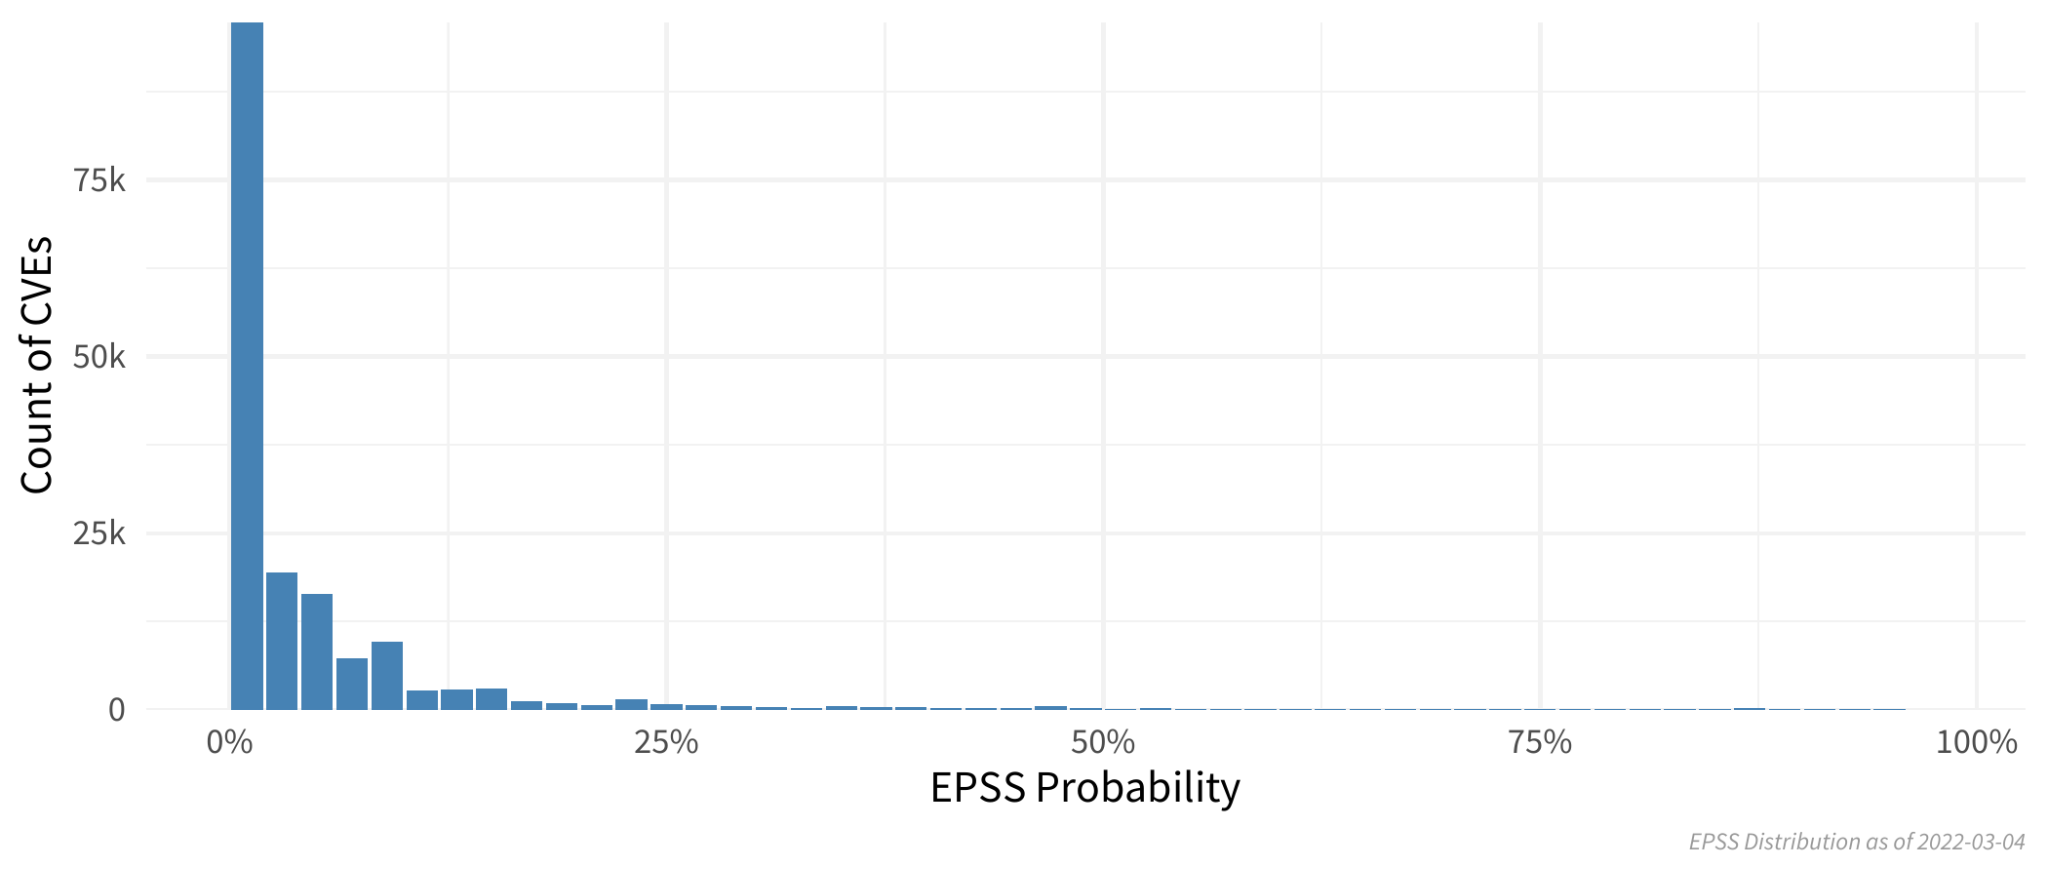
\includegraphics[width=\textwidth]{resources/EPSS_Prob_Dist.png}
    \caption{Distribution of \ac{EPSS} probabilities as of 2022-03-04 \autocite{first_exploit_2022}.}
    \label{fig:epss-distribution}
\end{figure}

The visualized distribution highlights the role of \ac{EPSS} in guiding remediation strategies. By focusing on high-probability vulnerabilities, organizations can efficiently allocate their resources to address the most critical threats, reducing the likelihood of exploitation while maintaining operational security.

Within this thesis, the \texttt{first.org} \ac{EPSS} database is queried via the provided \ac{API} to retrieve exploit probability scores for each identified vulnerability. These scores are integrated into the multidimensional classification model, combining them with \ac{CVSS} technical severity to enhance prioritization accuracy (see section~\ref{sec:algorithm-classifications}).

\subsection{Other Vulnerability Databases}
\label{subsec:other-vulnerability-databases}

While databases such as the \ac{DST}\footnote{\url{https://security-tracker.debian.org/tracker/}} and the \ac{RHD}\footnote{\url{https://access.redhat.com/security/security-updates/cve}} also offer valuable insights for vulnerability management, they are not examined in detail in this thesis due to their limited scope and specific focus on particular software ecosystems. These databases primarily target vulnerabilities within their respective platforms  -  Debian-based and Red Hat systems  -  which can limit their general applicability across a wider range of software environments. The primary focus of this work is on vulnerability databases that provide broader, cross-platform coverage and have higher adoption rates across diverse development ecosystems. As such, databases like the \ac{NVD}, \ac{OSV}, and \ac{GAD} were selected for their comprehensive, ecosystem-agnostic data.

\section{Scientific Foundations of the Expert Questionnaire}
\label{sec:scientific-foundations-questionnaire}

The expert evaluation conducted within this thesis can be understood as a form of self-report methodology, as it depends on subjective judgments provided by experts based on their professional knowledge and experience. According to \textcite{lucas_richard_e_global_2006}, self-report methodologies require respondents to interpret questions, recall relevant information, form judgments, and convert these judgments into responses. These cognitive processes underline the importance of careful questionnaire design, as each step can be substantially influenced by question wording, format, and context, thereby affecting the validity of responses \autocite{lucas_richard_e_global_2006}.

Further, as \textcite{schwarz_self-reports_1999} notes, respondents infer the pragmatic meaning of questions using contextual clues, including explicit framing provided by the questionnaire. Clearly specifying the context of the questionnaire as an expert evaluation conducted within a master's thesis on cybersecurity can thus guide respondents toward relevant and meaningful responses, enhancing the methodological rigor and reliability of the results.

Therefore, careful attention to question wording, context specification, and clear framing is essential for ensuring the validity of the expert evaluation, which this work has explicitly considered in designing the structured questionnaire.

The structured questionnaire used for the evaluation is presented in Appendix~\ref{appendix:questionnaire}.

\section{Lessons Learned from Existing Tools and \\ Their Impact on the Proposed Approach}
\label{sec:lessons-from-tools}

The literature review of current vulnerability management tools (refer to section~\ref{sec:multidimensional-approaches-tools}) shows that leading solutions adopt a multidimensional approach to vulnerability detection, assessment, and remediation. This approach is essential because vulnerabilities vary significantly in their characteristics and impacts, necessitating a comprehensive framework to effectively manage them. The following summary consolidates the scoring factors employed by prominent tools such as Tenable, Rapid7, and Snyk into a concise and comparative overview. By highlighting their respective strengths and specific scoring dimensions, this overview informs the development of a robust, hybrid vulnerability management model.

\subsection*{Consolidated Scoring Factors}
\label{subsec:consolidated_scoring_factors}

\begin{table}[H]
	\centering
	\label{tab:consolidated_scoring_factors}
	\begin{tabular}{|p{3.5cm}|p{3.2cm}|p{3.2cm}|p{3.2cm}|}
		\hline
		\textbf{Scoring Factor}               & \textbf{Tenable}               & \textbf{Rapid7}               & \textbf{Snyk}                   \\ \hline
		Technical Severity (CVSS)             & Yes & Yes & Yes                             \\ \hline
		Exploit Availability \& Maturity      & Yes (VPR)                      & Yes (honeypot data)    & Yes                             \\ \hline
		Threat Intelligence                   & Yes                            & Yes              & No                              \\ \hline
		Business Context \& Asset Criticality & Yes                            & Yes                           & No                              \\ \hline
		Exposure                              & No                             & Yes                           & No                              \\ \hline
		Fix Availability \& Vulnerability Age & Yes (vulnerability age) & No                            & Yes (patch availability) \\ \hline
		Additional Data Sources               & Yes (internal DB)       & Yes (partner data)     & Yes (public/internal DB) \\ \hline
	\end{tabular}
    	\caption{Consolidated Scoring Factors used by Tenable, Rapid7, and Snyk}
\end{table}

\subsection*{Summary and Impact on the Proposed Approach}
\label{subsec:summary_impact}

Insights from Tenable, Rapid7, and Snyk highlight the need for a multidimensional approach to vulnerability management that integrates technical severity with real-world exploit likelihood. A notable limitation of relying solely on \ac{CVSS} is scoring inconsistency, which can cause misaligned remediation priorities \autocite{spring_time_2021}.

Integrating the quantitative severity assessment provided by \ac{CVSS} with the probabilistic predictions from \ac{EPSS} into a unified scoring system addresses this issue. This hybrid model incorporates factors such as vendor intelligence, vulnerability age, exploit availability, exploit maturity, and threat intelligence, which are dimensions successfully utilized by Tenable, Rapid7, and Snyk (see section~\ref{subsec:consolidated_scoring_factors}). The studies conducted by \textcite{jacobs_exploit_2021} and \textcite{first_epss_2021} confirm that incorporating threat-likelihood metrics alongside \ac{CVSS} improves remediation efficiency by reducing patch workloads while effectively mitigating actively exploited vulnerabilities.

Using \ac{EPSS} and \ac{CVSS} together significantly enhances prioritization: \ac{CVSS} quantifies the \emph{impact} of vulnerabilities, while \ac{EPSS} estimates their \emph{likelihood of exploitation} based on empirical data.

Figure~\ref{fig:epss_cvss_compare} illustrates this concept clearly, showing the relationship between \ac{EPSS} probabilities and \ac{CVSS} scores for vulnerabilities as of 2021-05-16.

\begin{figure}[H]
	\centering
	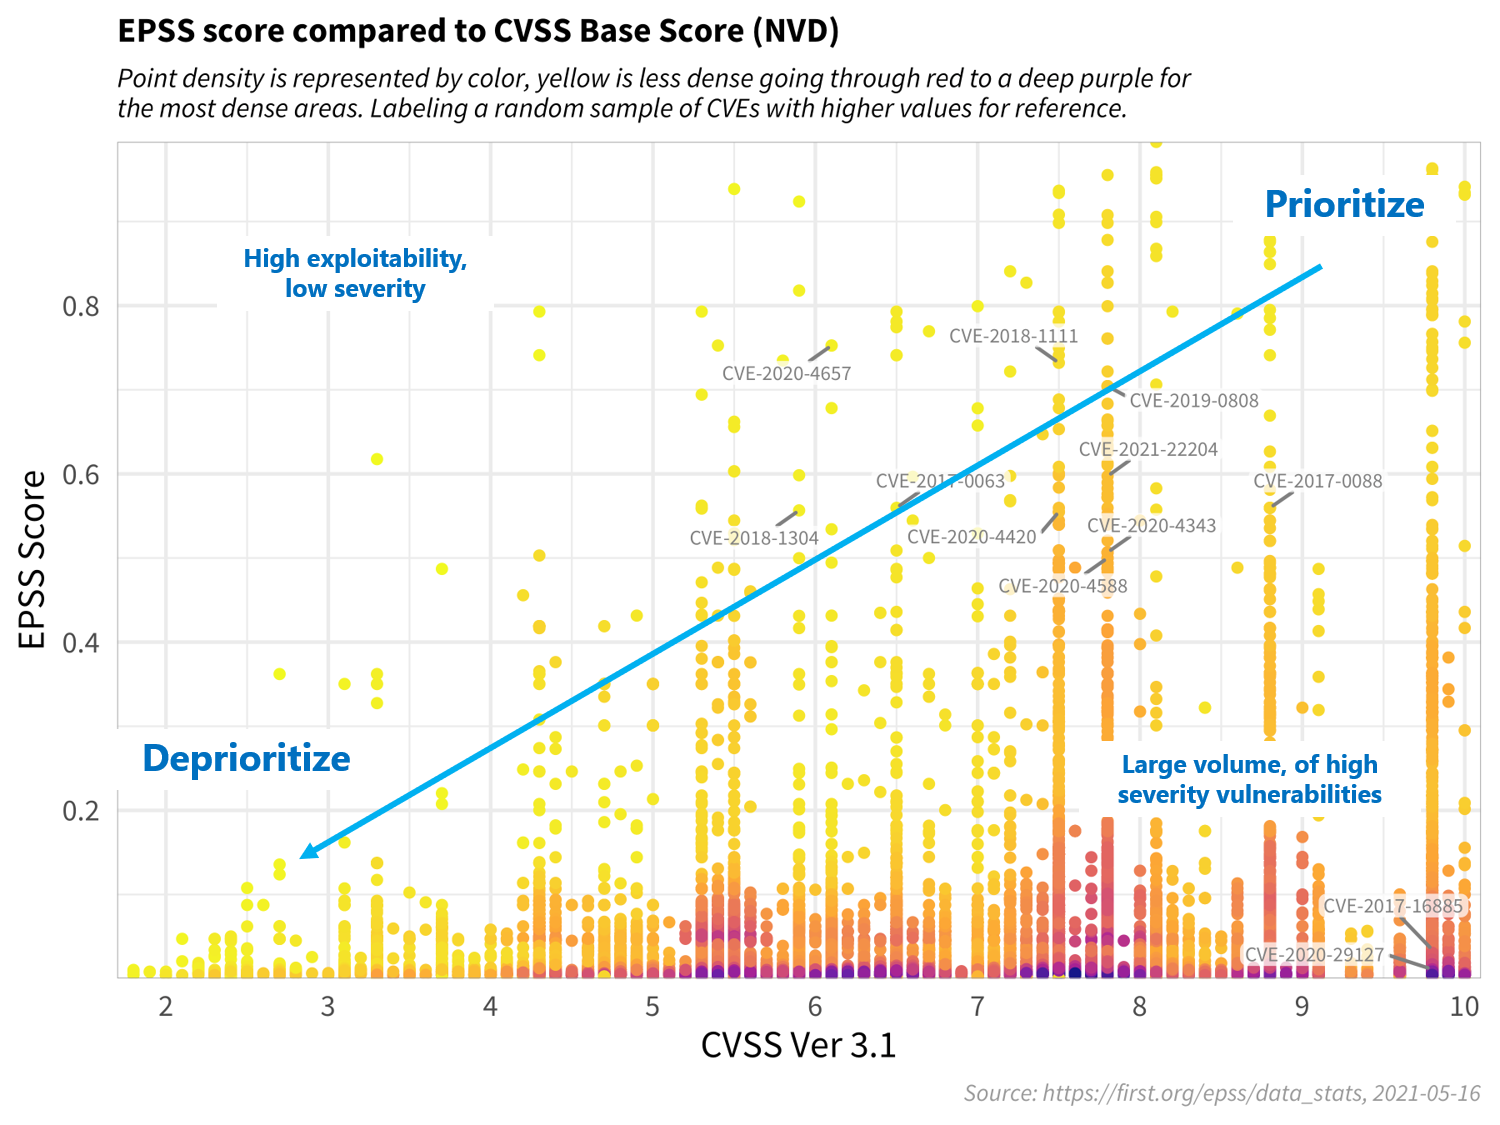
\includegraphics[scale=0.46]{resources/EPSS_CVSS_Compare.png}
	\caption[\ac{EPSS} and \ac{CVSS} Comparison]{Illustration of how \ac{EPSS} probabilities and \ac{CVSS} severity scores complement each other for better risk-based prioritization \autocite{first_epss_2021}.}
	\label{fig:epss_cvss_compare}
\end{figure}

Most vulnerabilities cluster towards lower exploit probabilities. Only a small fraction of vulnerabilities have \ac{EPSS} scores above 0.5. Although there is some correlation between \ac{EPSS} and \ac{CVSS} scores, this visualization clearly indicates that attackers do not exclusively target vulnerabilities that produce the greatest impact or are necessarily the easiest to exploit.

For prioritization, vulnerabilities in the lower-left quadrant (low probability, low impact) can typically be deprioritized. Vulnerabilities in the upper-left quadrant (high exploit probability, low impact) should be evaluated further, particularly in chained attack scenarios. Those in the lower-right quadrant (low exploit probability, high impact) warrant monitoring due to potential future exploitability. Vulnerabilities in the upper-right quadrant represent the highest risks (high probability, high impact) and must be addressed first \autocite{first_epss_2021}.

After establishing this combined severity score, the thesis applies a decision tree for remediation planning, drawing on the \ac{SSVC} framework (see section \ref{subsec:stakeholder-specific-vulnerability}). This tree incorporates \emph{Vulnerability Classification}, \emph{Patch Availability}, \emph{System Usage} (public or internal), \emph{Asset Criticality}, \emph{Fix Complexity}, \emph{Personal Code Ownership}, \emph{Exploit Likelihood}, \emph{Observed Exploits}, \emph{Compliance Requirement}, and \emph{Business Impact}. The required input data for these parameters is collected through a user query in the frontend, ensuring that context-specific factors are considered in the decision-making process. 

By blending a robust quantitative metric with a well-defined remediation process, the proposed framework addresses all of the key data considerations employed by Tenable, Rapid7, and Snyk - ensuring precise prioritization and more informed remediation strategies for critical vulnerabilities.
\chapter{Requirements}
\label{chapter:requirements}

This chapter defines the requirements for the multidimensional vulnerability classification and remediation system developed in the context of this master's thesis. Requirements are clearly structured and categorized into functional and non-functional requirements.

\section{Functional Requirements}
The functional requirements specify the necessary capabilities and behaviors the system must deliver to users.

\begin{enumerate}
	
	\item \label{req:multidimensional_classification}
	    \textbf{Multidimensional Vulnerability Classification Model:} The system shall provide a model capable of classifying vulnerabilities across multiple relevant dimensions, considering technical and empirical factors.
	      
	\item \label{req:classification_algorithm}
	      \textbf{Algorithm for Computing Vulnerability Classifications:} The system shall include an algorithm that computes a severity classification for vulnerabilities based on relevant and available data sources.
	      
	\item \label{req:remediation_algorithm}
	      \textbf{Remediation Recommendation Algorithm:} The system shall provide an algorithm to generate tailored recommendations for vulnerability remediation, taking into account factors such as stakeholder roles, asset importance, and patch availability.
	      
	\item \label{req:vulnerability_ranking_model}
	      \textbf{Rank-Ordering Model for Vulnerabilities:} The system shall provide a ranking model that prioritizes vulnerabilities according to their calculated severity, ensuring critical vulnerabilities receive immediate attention.
	      
	\item \label{req:interactive_explanation}
	      \textbf{Interactive Score Explanation Interface:} The system's user interface shall offer an interactive component that clearly explains how each vulnerability's overall severity was determined from underlying metrics.
	      
	\item \label{req:missing_data_handling}
	      \textbf{Handling of Missing Vulnerability Data:} When critical data required for scoring is unavailable, the system shall assign a placeholder score and clearly mark such vulnerabilities as having unknown severity.
	      
	\item \label{req:frontend_warning_missing_data}
	      \textbf{User Interface Warning for Missing Data:} The system shall explicitly inform users via the interface when necessary data is missing.
	      
	\item \label{req:ssvc_decision_tree}
	      \textbf{Role-Based Decision Trees for Remediation:} The system shall incorporate structured decision trees to provide customized remediation recommendations tailored to different stakeholder roles.
	      
	\item \label{req:role_specific_recommendations}
	      \textbf{Role-Specific Recommendations:} The system shall support various stakeholder roles, such as developers and security coordinators, by providing recommendations relevant to their specific responsibilities.
	      
	\item \label{req:data_caching_mechanism}
	      \textbf{Caching Mechanism for External Data:} The system shall implement caching for external vulnerability data to reduce unnecessary network requests and ensure efficient data retrieval.
	      
	\item \label{req:data_synchronization}
	      \textbf{Regular Data Synchronization:} The system shall perform regular synchronization with external vulnerability databases, maintaining updated and accurate vulnerability information.
	      
\end{enumerate}

\section{Non-Functional Requirements}
The non-functional requirements define quality criteria, constraints, and operational guidelines that the system must fulfill.

\begin{enumerate}
	
	\item \label{nfr:modularity}
	      \textbf{Modularity:} The system architecture shall be modular, distinctly separating functions such as data management, scoring computation, caching, and interface interaction to enhance maintainability.
	      
	\item \label{nfr:scalability}
	      \textbf{Scalability:} The system must be scalable to accommodate increased data volumes and user interactions without performance degradation.
	      
	\item \label{nfr:usability}
	      \textbf{Usability:} The user interface shall be intuitive, user-friendly, and provide clear guidance to ensure efficient and effective user interaction.
	      
	\item \label{nfr:rate_limit_compliance}
	      \textbf{Compliance with External API Rate Limits:} The system must manage external API requests responsibly, using strategies such as batching and caching to comply with rate limits and handle errors gracefully.
	      
	\item \label{nfr:reliability_fallbacks}
	      \textbf{Reliability and Error Handling:} Robust error handling mechanisms shall be implemented to maintain reliable system operation and clearly communicate any issues or missing information to users.
	      
	\item \label{nfr:maintainability}
	      \textbf{Maintainability:} The system design shall follow clear separation of concerns, facilitating straightforward modifications, updates, or integration of additional functionalities.
	      
\end{enumerate}

The functional and non-functional requirements presented in this chapter collectively define the essential attributes and capabilities necessary to build a robust and effective system for vulnerability management, emphasizing key aspects such as modularity, scalability, usability, and transparency.


\chapter{Multidimensional Vulnerability \\ Classification and Remediation Framework}
\label{chapter:multidimensional-vulnerability-classification}

This chapter introduces a multi-dimensional framework for classifying and remediating vulnerabilities by integrating factors such as exploit predictability, vulnerability age, and attack complexity. Drawing directly from the conclusions of the literature review (chapter~\ref{chapter:literature-review}) and the summarized insights in section~\ref{subsec:summary_impact}, the proposed approach addresses current limitations of the \ac{SCA} Tool developed by the \ac{FAU} Professorship for Open Source Software (\ac{OSS}), which classifies vulnerabilities exclusively based on \ac{CVSS} scores \autocite{nehrke_webdienst_2023}. Known limitations of this approach include inconsistent scoring among security professionals and its lack of empirical data on exploitability \autocite{spring_time_2021, jacobs_exploit_2021}. To enhance vulnerability classification, the proposed framework combines \ac{CVSS} severity scores with empirical exploit probability data provided by \ac{EPSS}.
For remediation prioritization, the stakeholder-specific \ac{SSVC} decision framework is employed, leveraging context-sensitive factors including asset criticality, fix complexity, and personal code ownership.

The chapter covers:
\begin{itemize}
    \item A model for multi-dimensional classification that evaluates vulnerabilities across multiple factors.
    \item An algorithm for computing classifications in specific software contexts.
    \item An algorithm for remediation recommendations tailored to stakeholders and asset criticality.
    \item A ranking model to prioritize vulnerabilities efficiently.
\end{itemize}

This framework aligns vulnerability management with both immediate and strategic security goals, addressing the complexities of modern software environments.

\section{A Model for Multi-Dimensional Classification of Vulnerabilities}
\label{sec:multi-dimensional-classification}

The following multi-dimensional classification model integrates several key dimensions to address both technical severity and real-world implications. Each dimension contributes to a holistic severity assessment; the dimensions used are:

\begin{itemize}
    \item \ac{CVSS} Score: Assesses technical severity using Version 3.1, which refines metrics and standardizes guidelines for comparability across systems (see section \ref{par:cvss-v3_1}). It considers factors like the attack vector, complexity, and the potential impacts on confidentiality, integrity, and availability.
    \item \ac{EPSS} Score: Represents the likelihood of real-world exploitation, based on empirical threat intelligence, such as publicly available exploits and observed attack trends.
\end{itemize}

As outlined in section~\ref{subsec:summary_impact}, \ac{CVSS} alone has been criticized for overlooking contextual factors and exhibiting scoring inconsistencies of 2--4 points among practitioners \autocite{spring_time_2021}. To address these gaps, \ac{EPSS} is incorporated as a complementary metric, leveraging real-world exploitation data to provide a more dynamic, threat-focused perspective. By combining \ac{CVSS}'s standardized impact assessment with \ac{EPSS}'s empirical likelihood estimations, this approach facilitates more context-aware remediation prioritization and aligns with industry best practices (see section~\ref{sec:multidimensional-approaches-tools}). This synergy ensures that vulnerabilities with both high severity and a proven likelihood of exploitation receive immediate attention, while those posing lower real-world risk can be deprioritized, leading to more efficient allocation of remediation resources.

These dimensions form the foundation of the classification model used to evaluate vulnerabilities. By integrating standardized technical scoring with real-world exploitability data, this approach balances static severity metrics with dynamic threat intelligence and ensures that both long-term structural risks and immediate threats are considered. However, some organizations may need to factor in additional internal criteria - such as extended liability or compliance requirements - that lie beyond the scope of \ac{CVSS} and \ac{EPSS}.

\section{Algorithm for Computing Classifications}
\label{sec:algorithm-classifications}

The classification algorithm prioritizes vulnerabilities by combining these dimensions, resulting in a tailored severity score that reflects both technical severity and real-world implications:

\begin{enumerate}
    \item \textit{Input Retrieval:} Gather data for each vulnerability, including \ac{CVSS} and \ac{EPSS} scores.

    \item \textit{Score Calculation:} Combine standardized technical scores \ac{CVSS} with real-world exploitability data \ac{EPSS} by multiplying the \ac{EPSS} probability value by 10.0 to align it with the 0--10 \ac{CVSS} range. The overall severity score is then obtained using the following weighted formula:

\begin{align*}
\text{Severity Score} 
&= \mathrm{round}\Biggl(
    \frac{
        w_{\text{cvss}} \times \text{CVSS}
        + w_{\text{epss}} \times \bigl(10.0 \times \text{EPSS}\bigr)
    }{2.0}
\Biggr)
\end{align*}

    where each weight \( w \) is configured to reflect organizational priorities or estimations by domain experts.

    \item \textit{Classification and Output:} Each vulnerability is assigned a classification (e.g., Critical, High, Medium, or Low) based on the calculated score. This final output serves as guidance for prioritizing vulnerabilities and improving the overall security posture.
\end{enumerate}

This work adopts a weighting factor of 2 for \ac{EPSS}, deliberately emphasizing empirical exploit probability. Because the calculation of \ac{EPSS} scores inherently incorporates certain elements from \ac{CVSS} base metrics - such as exploitability characteristics - assigning a higher weight to \ac{EPSS} emphasizes real-world exploitation likelihood while still effectively capturing the underlying technical severity. This approach ensures that vulnerabilities most likely to be actively exploited are prioritized, aligning vulnerability management closely with empirical evidence rather than purely theoretical severity assessments.

\subsection{Data Sources for the Classification Model}
\label{subsec:classification-data-sources}

The model integrates data from multiple sources to comprehensively evaluate vulnerabilities. Each vulnerability is referenced through a standardized \ac{CVE} identifier, enabling consistent data retrieval. Additional metrics, such as technical severity from \ac{CVSS} and empirical exploitation likelihood from \ac{EPSS}, are obtained through this identifier. The primary data sources include the \ac{NVD}, \ac{OSV}, \ac{GAD}, and the \texttt{first.org} \ac{EPSS} database.

\subsection{Handling Of Missing Data}
\label{subsec:handling-missing-data}

If the data required for calculating the severity score (see section \ref{sec:algorithm-classifications}) is missing, the algorithm assigns a default value of \textbf{10.1}. This placeholder score is not displayed to the user. Instead, the frontend labels the severity in pink as “UNKNOWN”, indicating that the severity could not be calculated. Since the maximum severity score is 10.0, a placeholder value of \textbf{10.1} ensures that the vulnerability is listed first on the dashboard.

\subsection{User Interface for Explaining Score Calculation and Guidance in Case Of Missing Data}
\label{subsec:ui-explaining-score}

To enhance the user’s understanding of the vulnerability scoring and prioritization, the system includes an interactive explanation feature and a method for handling incomplete data:

\textbf{Score Details Button:} The "Show Score-Details" button in the user interface provides detailed information about the calculated score. When clicked, it displays the following details:
    \begin{itemize}
        \item \textbf{\ac{CVE} ID:} Shows the \textit{Common Vulnerabilities and Exposures ID}, a unique identifier for the vulnerability. It helps security professionals track and reference the issue across different platforms and databases.
        \item \textbf{\ac{CVSS} Score (v3.1):} Displays the \textit{Common Vulnerability Scoring System} score, representing the severity of the vulnerability on a scale from 0.0 to 10.0. Higher scores indicate more critical vulnerabilities.
        \item \textbf{\ac{CVSS} Vector:} Provides the \textit{\ac{CVSS}} vector string, which describes the characteristics of the vulnerability, such as attack vector, attack complexity, and privileges required for exploitation.
        \item \textbf{\ac{EPSS} Score:} Shows the \textit{Exploit Prediction Scoring System} score, which estimates the likelihood of the vulnerability being exploited in the wild.
        \item \textbf{Severity Score:} Displays the overall severity score, calculated based on the combination of the \textit{\ac{CVSS}} Score and \textit{\ac{EPSS}} Score. This score helps prioritize remediation efforts effectively.
        \item \textbf{Hover Tooltips for Vectors:}  
        Displays hover-based tooltips for each \textit{\ac{CVSS}} vector attribute. When the user places the cursor over a specific field (e.g., “Attack Vector” or “Attack Complexity”), a concise explanation appears to clarify its impact on the vulnerability assessment.
        \item \textbf{Direct Link to the CVSS Calculator:}  
        A direct link to a prefilled \textit{\ac{CVSS}} calculator, ensuring that users can quickly review the existing \textit{\ac{CVSS}} metrics. This link is automatically populated with the relevant vector data, allowing rapid exploration of different scoring scenarios.
    \end{itemize}

\textbf{Guidance in Case Of Missing Data:}
\label{guidance-missing-data}
For cases where specific scores or recommendations are unavailable, the system transparently indicates missing components to the user. If critical data, such as the severity score, cannot be computed due to missing \ac{EPSS} or \ac{CVSS} scores, the user interface displays a clear red warning message stating: \textit{"Cannot compute: missing \ac{EPSS} or \ac{CVSS} Score! Remediation Strategy: Please run the \ac{SSVC} Assignment for further instructions!"} Additionally, the score details section may show placeholders like “\ac{CVSS}: N/A” to inform users that certain information was not included in the score calculation, thus ensuring transparency.

This approach ensures that users are fully informed about how each vulnerability score is calculated, providing transparency and clarity. Additionally, handling missing data with fallback messages maintains consistency in user experience and supports informed decision-making, even when data is incomplete.

\section{A Model for Remediation Recommendation}
\label{sec:remediation_recommendation}

This section presents the \ac{SSVC} vulnerability prioritization methodology, which leverages the \ac{SSVC} framework to generate tailored remediation recommendations through structured decision trees. These decision trees guide stakeholders, such as developers and security advisors, in determining the most appropriate remediation actions for each vulnerability.

The \ac{SSVC} framework, as discussed in section~\ref{subsec:stakeholder-specific-vulnerability}, does not directly affect the vulnerability score but guides remediation by aligning recommendations with organizational priorities. As outlined in section~\ref{subsec:summary_impact}, it mirrors industry solutions (e.g., Tenable, Rapid7, Snyk) by factoring in elements such as \emph{Exploit Status}, \emph{Exposure}, \emph{Asset Criticality}, and \emph{Patch Availability}. The \ac{SSVC}-based decision tree incorporates these parameters, gathered via a frontend user query, to ensure context-informed remediation.

Using the decision trees, vulnerabilities are categorized and prioritized for immediate patching, monitoring, or deprioritization. An example of such a decision tree tailored specifically to developers is illustrated in figure~\ref{fig:ssvc-remediation-developer}. For instance, if the exploit likelihood is high and a patch is available, developers should apply the patch immediately. If no patch is available, regular monitoring is recommended. Conversely, vulnerabilities with low exploit likelihood affecting non-critical assets can be deprioritized.

\begin{figure}[H]
\centering
\resizebox{0.6\textwidth}{!}{
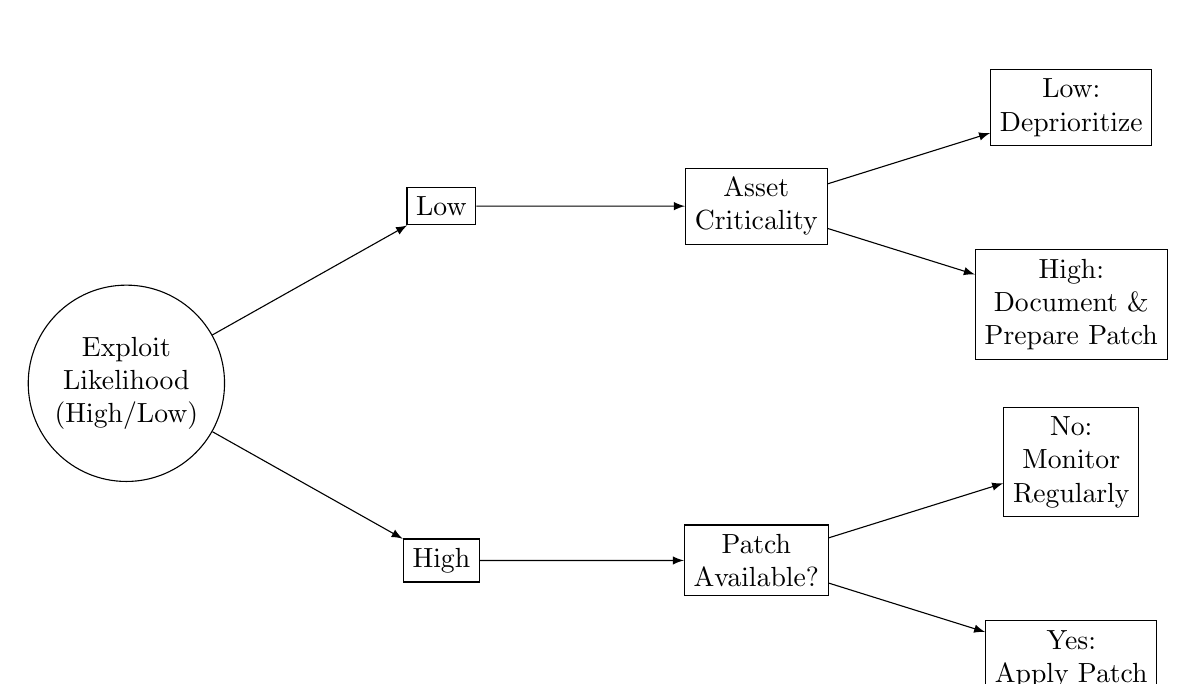
\begin{tikzpicture}[
    grow=right,
    level distance=40mm,
    level 1/.style={sibling distance=45mm},
    level 2/.style={sibling distance=45mm},
    edge from parent/.style={draw, -latex},
    node distance=1cm
]
\node [circle, draw, align=center] {Exploit\\Likelihood\\(High/Low)}
    child {
        node [rectangle, draw, align=center] {High}
        child {
            node [rectangle, draw, align=center] {Patch\\Available?}
            child [yshift=+10mm] {
                node [rectangle, draw, align=center] {Yes:\\Apply Patch}
            }
            child [yshift=-10mm] {
                node [rectangle, draw, align=center] {No:\\Monitor\\Regularly}
            }
        }
    }
    child {
        node [rectangle, draw, align=center] {Low}
        child {
            node [rectangle, draw, align=center] {Asset\\Criticality}
            child [yshift=+10mm] {
                node [rectangle, draw, align=center] {High:\\Document \&\\Prepare Patch}
            }
            child [yshift=-10mm] {
                node [rectangle, draw, align=center] {Low:\\Deprioritize}
            }
        }
    };
\end{tikzpicture}
}
\caption{Example of an \ac{SSVC} Decision Tree for Remediation Recommendations for the Developer Role}
\label{fig:ssvc-remediation-developer}
\end{figure}

By applying this structured approach, the \ac{SSVC} methodology ensures that remediation decisions align closely with stakeholder priorities and operational context, improving resource allocation and enabling more effective management of vulnerabilities.

\section{Algorithm for Remediation Recommendation}
\label{sec:algorithm-remediation}

This algorithm provides remediation recommendations based on the \ac{SSVC} model. By considering factors such as stakeholder roles (e.g., developers, security coordinators), \emph{Patch Availability}, and \emph{Asset Criticality}, the algorithm generates tailored actions to address vulnerabilities efficiently. The following steps outline the decision-making process for each vulnerability:

\begin{enumerate}
    \item \textit{Input Retrieval and Initial Assessment:}  
    The algorithm collects essential information about each vulnerability (e.g., the data points listed below), though in practice additional parameters may also be gathered to capture further contextual details:
    \begin{itemize}
        \item \emph{Stakeholder Role} to identify the responsibilities and potential impact for each user type, e.g., developers, operators, or security coordinators.
        \item \emph{Asset Criticality} to determine the priority based on the business importance of the affected asset.
        \item \emph{Patch Availability} to inform the urgency and feasibility of the remediation.
    \end{itemize}

    \item \textit{\ac{SSVC}-Based Decision Tree for Remediation Action:} The algorithm uses \ac{SSVC}-inspired decision trees tailored to the roles of different stakeholders. In this example, the stakeholders include developers and security coordinators, each of whom receives specific recommendations based on their roles and responsibilities. This ensures that each role receives appropriate remediation guidance based on the specific characteristics of the vulnerability. Example actions for each stakeholder include:
    \begin{itemize}
        \item \textbf{Developers:}
            \begin{itemize}
                \item \textbf{High Exploit Likelihood and Patch Available:} Apply patch immediately to prevent exploitation.
                \item \textbf{High Exploit Likelihood and No Patch Available:} Document the vulnerability, monitor regularly, and prepare for a future patch.
                \item \textbf{Low Exploit Likelihood and Critical Asset:} Prepare patch documentation; consider patching in the next scheduled maintenance.
            \end{itemize}
        \item \textbf{Security Coordinators:}
            \begin{itemize}
                \item \textbf{High Exploit Likelihood and Critical Asset:} Initiate immediate response, notify relevant teams, and enforce monitoring.
                \item \textbf{Low Exploit Likelihood and Non-Critical Asset:} Document vulnerability details and set a reminder for review in future security audits.
                \item \textbf{Significant Stakeholder Impact:} Prepare backup and documentation for affected systems, even if exploit likelihood is low, to ensure preparedness.
            \end{itemize}
    \end{itemize}

    \item \textit{Classification of Recommended Actions:} Based on the outputs of the \ac{SSVC}-based decision tree, each vulnerability is assigned a recommended action classification, such as:
    \begin{itemize}
        \item \textbf{Immediate Patch}: High-priority vulnerabilities with available patches are recommended for immediate remediation.
        \item \textbf{Monitor and Prepare Patch}: Vulnerabilities with no immediate fix, but high exploit likelihood, are recommended for regular monitoring and preparation for a patch.
        \item \textbf{Deprioritize}: Low-priority vulnerabilities affecting non-critical assets and posing minimal exploit risk are deprioritized but documented for future reference.
    \end{itemize}

    \item \textit{Output of Recommendations:} The algorithm generates the recommended remediation actions for each vulnerability, taking into account the specific roles and priorities of each stakeholder. The recommendation provides a comprehensive view of immediate actions, monitoring tasks, and deprioritized items, ensuring that resources are allocated effectively to mitigate high-risk vulnerabilities.
\end{enumerate}

This algorithm enables context-sensitive and efficient vulnerability management by aligning recommended actions with the needs of different stakeholders, such as developers and security coordinators, as well as the operational importance of each asset. This ensures that the most critical vulnerabilities are addressed promptly, while lower-risk issues are monitored or deprioritized.

\section{A Model to Rank-Order All Classified Vulnerabilities}
\label{sec:rank-order-vulnerabilities}

This model provides a structured approach for ranking all known vulnerabilities based on their calculated scores, prioritizing those with the highest severity to ensure efficient allocation of resources. By leveraging the composite scores generated through the multi-dimensional classification model, this ranking mechanism enables organizations to address the most critical vulnerabilities first. The steps for implementing this ranking model are outlined as follows:

\begin{enumerate}
    \item \textbf{Score Aggregation:} 
    The total score for each vulnerability is calculated from the weighted dimensions \ac{EPSS} and \ac{CVSS} (see section \ref{sec:algorithm-classifications}). This score provides a unified measure of severity.
    
    \item \textbf{Handling Missing Data (Default Score 10.1):} 
    When essential data for scoring is unavailable, the algorithm assigns a placeholder score of \textbf{10.1} - exceeding the maximum valid severity of 10.0 (see section \ref{subsec:handling-missing-data}). In the user interface, this appears as a pink \textbf{“UNKNOWN”} label rather than the numeric score, ensuring it is displayed first in the dashboard and prompting immediate attention to gather the missing information.
    
    \item \textbf{Sorting and Rank-Order Calculation:} 
    All classified vulnerabilities are sorted in descending order of their total (or placeholder) score, with the highest scores - whether valid or placeholder - representing the most urgent cases.
    
    \item \textbf{Resource Allocation Guidance:} 
    Based on the ranked list, organizations can allocate resources toward the vulnerabilities that pose the highest risk. This enables a focused remediation effort, ensuring that the most severe or unknown-risk vulnerabilities are addressed first.
    
    \item \textbf{Dynamic Re-Ranking Based on Score Changes:} 
    If there are updates to any of the vulnerability scores - such as new threat intelligence or changes in asset criticality - the model recalculates and reorders the list to reflect the latest context, keeping the priority list up-to-date.
\end{enumerate}

This ranking model complements the multi-dimensional classification and remediation framework by establishing a clear, actionable prioritization order. It ensures that both high-risk and data-incomplete vulnerabilities are addressed promptly, aligning with strategic security objectives and operational capacity.
\chapter{Design}
\label{chapter:design}

This chapter describes the current and proposed designs for managing vulnerability data, emphasizing scalability and efficient interaction between system components. Building on the multidimensional classification and remediation model outlined in chapter \ref{chapter:multidimensional-vulnerability-classification}, the proposed extension translates these concepts into a scalable and practical system design.

\section{Current Design}
\label{sec:current-design}

The current solution integrates data from the \ac{OSV} database into the internal system for vulnerability management. This process ensures efficient synchronization, processing, and storage of vulnerability advisories, aligning these advisories with components specified in the \ac{SBOM} to identify packages and components affected by vulnerabilities.

\begin{itemize}
    \item \textbf{Data Synchronization:} The system initiates synchronization by checking for the availability of the vulnerability data archive (\ac{OSV}) in a cloud-based storage system. This includes mechanisms to verify the freshness of the data (e.g., through metadata such as ETags) to avoid redundant processing. Only updated or newly added archives are retrieved and temporarily stored for processing. This process happens once a day.

    \item \textbf{Data Extraction and Processing:} Retrieved archives are decompressed, and individual advisories are parsed and processed. Each advisory is evaluated for updates since the last synchronization and is enriched with relevant details, such as identifiers, severity metrics, and associated packages. 
    \begin{itemize}
        \item \textbf{Change Detection:} Only advisories that have been modified since the previous synchronization are processed further.
        \item \textbf{Mapping and Enrichment:} Relevant details, including affected components, vulnerability types, and risk metrics (e.g., \ac{CVSS}), are extracted and structured for database integration.
    \end{itemize}

    \item \textbf{Component Alignment:} Processed advisories are matched against the components listed in the \ac{SBOM}. This step identifies specific packages and software elements within the \ac{SBOM} that are directly affected by vulnerabilities, enabling precise vulnerability reporting at the component level.

    \item \textbf{Database Update:} The structured advisories, enriched with mappings to specific components, are stored in the internal database. Synchronization metadata, such as timestamps and version identifiers, is updated to reflect the latest state of external data sources. When an \ac{API} request is triggered, the relevant data is sent to the frontend, ensuring the user interface always reflects the most recent vulnerability information.
\end{itemize}

\section{Extended Design}
\label{sec:extended-design}

The extended design centers on a streamlined approach to vulnerability information management. It integrates multiple data sources (e.g., vulnerability databases, scoring providers) and applies caching to reduce unnecessary network requests. Its purpose is to unify critical metrics (such as \ac{CVSS}, \ac{EPSS}) into a consolidated view, as described in the multi-dimensional classification model (see section \ref{sec:multi-dimensional-classification}), while also supporting role-specific actions based on the remediation model outlined in section \ref{sec:remediation_recommendation}.

\subsection{Backend Responsibilities}
\label{subsec:backend-responsibilities}

The backend is responsible for data retrieval, caching, and score computation, following the scoring algorithm described in section \ref{sec:algorithm-classifications}:
\begin{itemize}
    \item \textbf{Multi-Source Lookup:}  
    For each vulnerability, the system first queries the \ac{OSV} database to retrieve both the \ac{CVE} identifier and (if available) the \ac{CVSS} vector, leveraging \ac{OSV}'s integration of the entire \ac{GAD}.\footnote{\url{https://osv.dev/}} If no \ac{CVSS} vector is found there, the system sends a request to external sources (e.g., the \ac{NVD}), thereby minimizing the number of lookups. Similarly, the system always retrieves \ac{EPSS} data from the \texttt{first.org} database to ensure it remains up to date, as it is not included in the internal \ac{OSV} cache.
    \item \textbf{Caching and Time-Based Retrieval:}  
    The system initiates a daily update cycle by first attempting to retrieve \ac{CVSS} vectors from its local \ac{OSV} database. If unavailable, it sends individual requests to the \ac{NVD} for the missing \ac{CVSS} details, as batch queries for \ac{CVE} IDs are not supported.\footnote{\url{https://nvd.nist.gov/developers/vulnerabilities}} Simultaneously, batch requests are sent to the \texttt{first.org} database for \ac{EPSS} scores.
    After retrieving the new information, the cache is refreshed and any derived metrics (e.g., severity) are recalculated.
    \item \textbf{Role-Specific Recommendations:} Based on user input (e.g., developer or security advisor), the system determines a recommended course of action (see section \ref{sec:remediation_recommendation}). The backend solely stores the \ac{SSVC} recommendation, which might include immediate patching, hotfixes, or a scheduled approach, for later retrieval or review.
\end{itemize}

\subsection{Frontend Responsibilities}
\label{subsec:frontend-responsibilities}

The frontend is responsible for fetching data from the backend, displaying it to the user, and forwarding user inputs for storage. Key functionalities include:

\begin{itemize}
  \item \textbf{View Scores and Vectors:} A dedicated interface fetches data from the backend and displays \ac{CVE} identifiers, \ac{CVSS} vectors, \ac{CVSS} base scores, \ac{EPSS} values, overall severity, and missing data, as described in section \ref{subsec:ui-explaining-score}. Additionally, it is responsible for showing vulnerabilities ranked as described in section \ref{sec:rank-order-vulnerabilities}.
  \item \textbf{Perform Structured Assignments:} An interactive decision flow guides users (depending on their role) through a series of questions, ultimately generating a recommendation, as seen in the concept of section \ref{sec:remediation_recommendation}. 
  \item \textbf{Send Updates to the Backend:} Once the recommendation is finalized, it is transmitted to the backend for persistence.
\end{itemize}


\subsection{System Interaction Workflow}
\label{subsec:system-interaction}

This section outlines the mechanisms for updating, fetching, and caching vulnerability data. Figure~\ref{fig:data-fetch-flow} shows how the process begins with a scheduled update (e.g., at midnight) or an \ac{API} request from the frontend. In the latter case, if the vulnerability entity exists, the system returns it immediately; otherwise, a new record is created, and the creation or update process continues.

The backend checks if a \ac{CVE} is in the cache. If not, the workflow transitions to an \texttt{Error} state, returning a severity score of \textbf{10.1} (see section~\ref{subsec:handling-missing-data}), highlighted in pink on the frontend. Users can consult the \emph{Score Explanation} feature (see section~\ref{subsec:ui-explaining-score}) for guidance. If the \ac{CVE} exists, the system checks whether \ac{CVSS} data is cached. If unavailable, an external fetch is performed. The \ac{EPSS} metric is always retrieved externally to ensure it remains up to date, as it is not included in the cache.

Failure in either fetch leads to the \texttt{Error} state, while successful retrieval allows the system to compute an overall severity score (see section~\ref{sec:algorithm-classifications}) and store the final data. The process concludes by returning a fully updated record to the caller.

\begin{figure}[H]
\centering
\caption{The internal data-fetching, caching, and updating workflow for vulnerability data.}
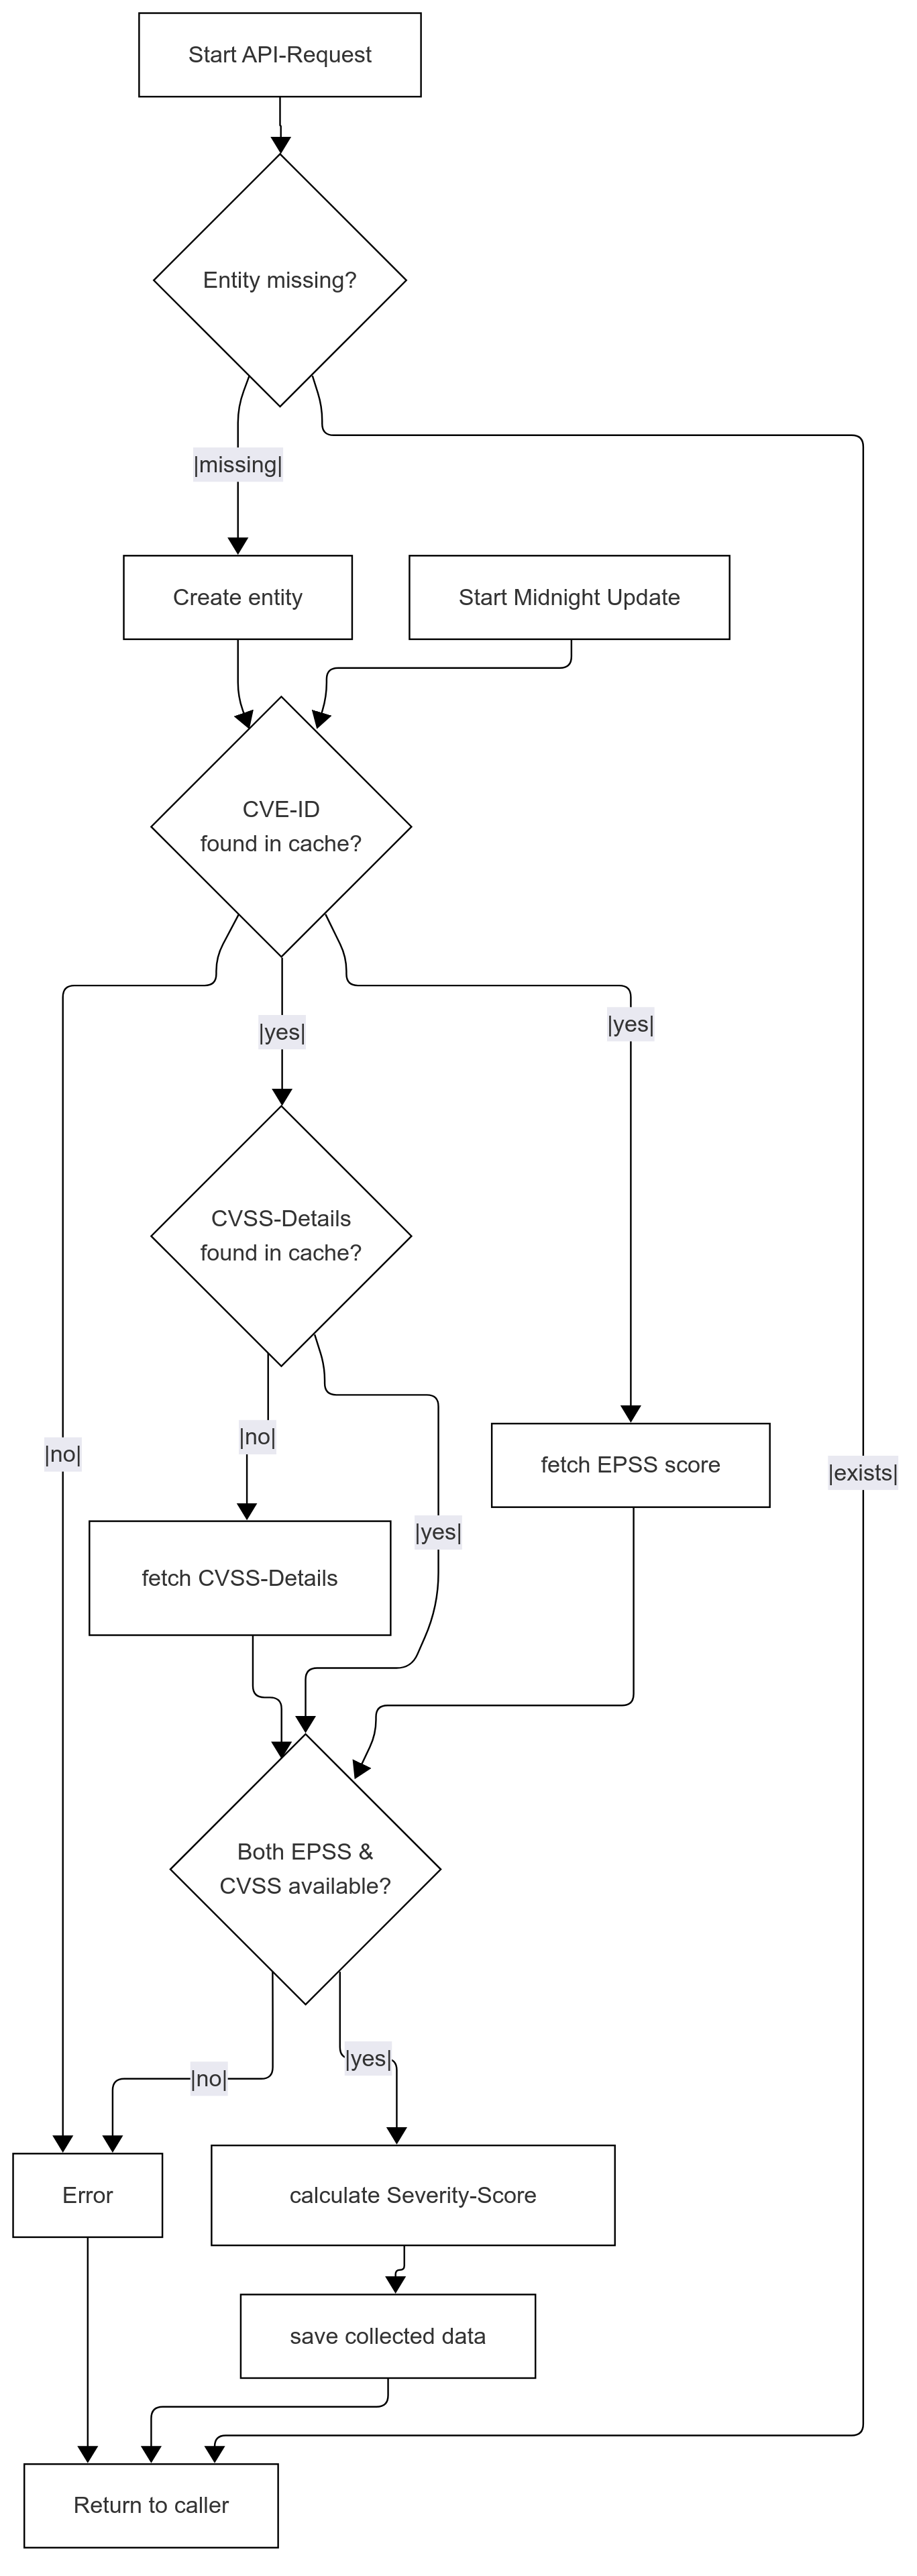
\includegraphics[width=1\textwidth,height=1\textheight,keepaspectratio]{resources/Data_Flow_Vulnerability_Data.png}
\label{fig:data-fetch-flow}
\end{figure}

\subsection{Rate Limits and Caching Benefits}
\label{subsec:rate-limits-caching}

In this design, \ac{CVE} data is exclusively retrieved from the local \ac{OSV} database, while \ac{CVSS} data is primarily obtained from the local \ac{OSV} database as well, querying the \ac{NVD} only if the required information is unavailable locally. Additionally, \ac{EPSS} data is fetched directly from \texttt{first.org}. External data sources impose rate limits to prevent misuse; for instance, the \ac{NVD} restricts queries to five requests per 30-second window without an \ac{API} key, and fifty with one.\footnote{\url{https://nvd.nist.gov/developers/start-here}} The \texttt{first.org} database enforces a threshold of 1,000 requests per hour without a token.\footnote{\url{https://api.first.org/\#Rate-Limit}} Since \ac{CVE} and most \ac{CVSS} data are retrieved locally from the \ac{OSV} database, no rate limits apply to these queries.

To cope with these constraints, the backend employs caching and batching to reduce repetitive lookups. Data retrieval occurs only when a record is missing or considered outdated, significantly minimizing external calls and reducing the risk of exceeding rate limits. During nightly updates, requests for \ac{EPSS} scores are processed in batches to further optimize efficiency. However, since the \ac{NVD} does not support batch queries for \ac{CVE} IDs,\footnote{\url{https://nvd.nist.gov/developers/vulnerabilities}} \ac{CVSS} data retrieval requires individual requests, making caching even more essential. Consequently, the system operates more reliably and gracefully handles errors by returning a severity score of \textbf{10.1} (see section~\ref{subsec:handling-missing-data}) whenever fetch errors occur. This condition is visually highlighted in pink on the frontend, prompting users to consult the score explanation interface (see section~\ref{subsec:ui-explaining-score}) to identify appropriate next steps for issue resolution.

\subsection{SSVC Process and Role-Specific Assignments}
\label{subsec:ssvc-process}

The \ac{SSVC} process involves tailoring vulnerability handling to each user's or team's specific context, following the stakeholder-specific prioritization framework described in section \ref{sec:algorithm-remediation}. This process is supported by the controller layer, which manages endpoints like the \ac{SSVC} recommendation endpoint. These endpoints facilitate the submission of role-specific decisions, which are then persisted and integrated with other metrics (e.g., \ac{CVSS}, \ac{EPSS}). Figure~\ref{fig:ssvc-interaction} illustrates this interaction.

\begin{figure}[H]
\centering
\resizebox{0.9\textwidth}{!}{%
\begin{tikzpicture}[>=stealth', node distance=2.5cm, auto, thick, font=\sffamily\small]

  \node[draw, rectangle, rounded corners, align=center, minimum width=3cm, minimum height=1cm] (frontend) {User Interface};
  \node[draw, rectangle, rounded corners, right=4.0cm of frontend, minimum width=3.3cm, align=center] (backendController) {Controller Layer};
  \node[draw, rectangle, rounded corners, right=3.5cm of backendController, minimum width=3.3cm, align=center] (backendStorage) {Data Storage \\ \& Calculation};

  \draw[->] (frontend.east)
    to[out=0, in=180]
    node[above, yshift=0.2cm]{\scriptsize Finalize Role-Based Decision}
    (backendController.west);

  \draw[->] (backendController.east)
    to[out=0, in=180]
    node[above, yshift=0.2cm]{\scriptsize Persist and Merge Data}
    (backendStorage.west);

  \draw[->] (backendStorage.south west)
    to[out=230, in=-50]
    node[below, yshift=-0.2cm]{\scriptsize Return Updated Metrics}
    (backendController.south east);

  \draw[->] (backendController.south west)
    to[out=230, in=-50]
    node[below, yshift=-0.2cm]{\scriptsize Updated Values (CVSS, EPSS, etc.)}
    (frontend.south east);

\end{tikzpicture}
}
\caption{High-level interaction in the \ac{SSVC} process.}
\label{fig:ssvc-interaction}
\end{figure}

\section{Conclusion}
\label{sec:design-conclusion}
The outlined design consolidates key vulnerability metrics and merges them with role-based inputs to yield tailored recommendations. By systematically checking internal data first and fetching new information only when required, it minimizes redundant requests while maintaining data accuracy. Frontend interactions are kept straightforward through specialized dialogs and status views, ensuring users can easily view or update vulnerability details. This approach offers a strong foundation for integrating further data sources and scaling to large application ecosystems.
\chapter{Implementation}
\label{chapter:implementation}

This chapter focuses on the implementation of the components proposed in section \ref{sec:extended-design}. It describes how the backend functionalities, such as caching mechanisms, data acquisition workflows, and the \ac{SSVC} recommendation process, were realized to ensure efficient data handling and seamless integration with external systems. Additionally, the chapter explains how the frontend was implemented to support user interactions, including role-specific remediation-strategies and data visualization. This implementation bridges the gap between architectural design and a functional, scalable system.

\section{Backend Components}
\label{sec:backend-components}

This section explains the main backend building blocks, focusing on data storage, retrieval logic, and the mechanisms used to ensure up-to-date information.

\subsection{Caching Mechanism and Repository Layer}
\label{subsec:caching-repository}

A central piece of functionality is the storage of previously retrieved data. Two core strategies are employed to manage data retrieval: \textbf{Pre-Check} and \textbf{Scheduled Refresh}.

The \textbf{Pre-Check} strategy involves querying the internal repository whenever a vulnerability request arises. The system first checks whether a corresponding \textit{Vulnerability Data Entity} already exists. If it does, the existing record is returned. If no such entry is found, the system creates a new entity while simultaneously checking the local \ac{OSV} database for the associated \ac{CVSS} vector. If the vector is not available locally, an external \ac{API} call to the \ac{NVD} is performed to retrieve the missing details. In parallel, the \ac{EPSS} score is fetched from the external \texttt{first.org} \ac{API}, as it is not stored locally (see section~\ref{subsec:backend-responsibilities}).

The \textbf{Scheduled Refresh} strategy ensures data freshness through a nightly update cycle. This process starts 30 minutes after the \ac{OSV} database update (see section ~\ref{sec:current-design}), ensuring that the most recent vulnerability information is available. During this cycle, the system updates the entire dataset by performing batch requests for \ac{EPSS} scores via the \texttt{first.org} \ac{API} and individual requests to the \ac{NVD} for missing \ac{CVSS} details not available in the local \ac{OSV} database, as the \ac{NVD} does not support batch queries for \ac{CVE} IDs.\footnote{\url{https://nvd.nist.gov/developers/vulnerabilities}}

If either the \ac{CVSS} or \ac{EPSS} data cannot be retrieved, the system transitions to an \texttt{Error} state, returning a severity score of \textbf{10.1}. This value is highlighted in pink on the frontend to prompt user action (see section~\ref{subsec:handling-missing-data}).

\noindent
\paragraph{Example of a Caching Strategy (Pseudocode)}
\label{par:example-caching-strategy}

\begin{verbatim}
// Caching Strategy Pseudocode

// Check if vulnerability exists
if (existsInRepository(cveId)) {
    return getFromRepository(cveId);
}

// Create new entity and fetch data
entity = createNewEntity(cveId);
entity.cvssVector = getFromOsv(cveId) ?? fetchFromNvd(cveId);
entity.epssScore  = fetchFromFirstOrg(cveId);

// Save and return entity
saveToRepository(entity);
return entity;
\end{verbatim}

\noindent
If any data retrieval fails, the process is aborted, and the system proceeds as described in section~\ref{subsec:handling-missing-data}.

\subsection{Scheduled Refresh Mechanism}
\label{subsec:scheduled-refresh}

The \textbf{Scheduled Refresh} strategy ensures data freshness through a nightly update cycle. This process starts 30 minutes after the \ac{OSV} database update, ensuring that the most recent vulnerability information is available.

During this cycle, the system iterates through all existing \textit{Vulnerability Data Entities} and updates each entry as follows:
\begin{itemize}
    \item The local \ac{OSV} database is queried for the latest \ac{CVSS} vector.
    \item If the vector is not found locally, an external \ac{API} call is made to the \ac{NVD}.
    \item In parallel, the \ac{EPSS} scores are fetched in a batch from the external \texttt{first.org} \ac{API}, as it is not cached locally.
\end{itemize}

If any data retrieval fails, the system aborts the update for the affected entry and proceeds as described in section~\ref{subsec:handling-missing-data}. Successfully updated entities are saved back to the repository, ensuring the dataset remains accurate and current.

\noindent
\paragraph{Daily Vulnerability-Data Update (Pseudocode)}
\label{par:daily-vulnerability-update-short}

\begin{verbatim}
// Scheduled job: runs daily at 00:30
scheduleRecurringTask("vulnerability-data-update", "0 30 0 * * *") {
    updateVulnerabilityData();
}

function updateVulnerabilityData() {
    // Fetch all vulnerabilities
    entities = vulnerabilityDataRepository.findAll();

    // Batch-fetch EPSS scores
    epssScores = fetchBatchEpssScores(collectCveIds(entities));

    // Update each entity
    for each entity in entities {
        entity.epssScore  = epssScores.get(entity.cveId);
        [entity.cvssScore, entity.cvssVector] =
        fetchCvssScoreAndVector(
            entity.cveId,
            entity.vulnId
    );
        entity.severityScore = calculateSeverityScore(entity);
        entity.severityScoreLastUpdated = now();

        // Save updated entity
        vulnerabilityDataRepository.save(entity);
    }
}
\end{verbatim}

\paragraph{SSVC Recommendation Endpoint}
\label{par:ssvc-recommendation-endpoint}

The \ac{SSVC} recommendation endpoint, part of the controller layer, allows the frontend to submit tailored remediation plans. As described in section \ref{subsec:ssvc-process}, this endpoint integrates role-specific decisions into the backend’s controller layer. These recommendations are stored in the backend for integration with other vulnerability metrics. The pseudo-implementation is as follows:

\noindent
\paragraph{Updating SSVC Recommendation (Pseudocode)}
\label{par:update-ssvc-recommendation}

\begin{verbatim}
// For a POST request to "/api/.../vulnerabilities/{vulnId}/ssvc"
function updateSsvc(vulnId, ssvcRecommendation):
    // Retrieve the vulnerability record by its ID
    data = repository.findById(vulnId)
    
    // If found, update recommendation and save
    if data:
        data.ssvcRecommendation = ssvcRecommendation
        repository.save(data)
    
    // Return success response
    return HTTP_200_OK
\end{verbatim}

This process ensures that:
\begin{itemize}
  \item \ac{SSVC} recommendations are properly stored for each vulnerability.
  \item The data is integrated with other metrics such as \ac{CVSS} and \ac{EPSS}.
  \item The recommendations are available for retrieval and analysis in future requests.
\end{itemize}

\subsection{Severity Score Calculation}
\label{subsec:severity-score}

After confirming the presence of \ac{CVSS}, \ac{EPSS}, and any other relevant metrics, the system generates a composite severity score. This calculation is based on the multi-dimensional classification model introduced in section \ref{sec:multi-dimensional-classification}, which integrates technical severity and real-world exploitability.

The algorithm follows the methodology described in section \ref{sec:algorithm-classifications}, prioritizing vulnerabilities by combining these metrics into a unified severity score. The specific steps are outlined as follows:

\begin{enumerate}
  \item \textbf{Validate Required Fields}: If either the \ac{CVSS} base score or \ac{EPSS} value is missing, log an error and default them to \textbf{10.1}.
  
  \item \textbf{Combine Weighted Values}: Multiply the \ac{EPSS} probability by 10.0 to make it numerically compatible with the \ac{CVSS} score (0--10).

  \item \textbf{Compute Weighted Severity Score}: Calculate the severity score using the following pseudocode:

  \begin{verbatim}
double epssScaled = epss * 10.0;
double severity = ((w_cvss * cvss) + (w_epss * epssScaled)) / 2.0;
severity = round(severity);
  \end{verbatim}

  Here, the weights \( w_{\text{cvss}} \) and \( w_{\text{epss}} \) follow the definitions provided in section \ref{sec:algorithm-classifications}, reflecting their relative importance in the overall severity assessment.

  \item \textbf{Store the Result}: Update the database record with the newly calculated severity score.
\end{enumerate}

\paragraph{Example of Combining \ac{CVSS} and \ac{EPSS}}
\label{par:cvss-epss-combination}
The following example demonstrates how \ac{CVSS} and \ac{EPSS} scores are combined to compute the severity score, aligning with the weighted scoring formula presented in section \ref{sec:algorithm-classifications}:
\noindent
\paragraph{Severity Score Calculation (Pseudocode)}
\label{par:severity-score-calculation}

\begin{verbatim}
// Calculate severity score based on CVSS and EPSS
function calculateSeverityScore(data):
    cvss = data.getCvssScore()  // 0.0 to 10.0
    epss = data.getEpssScore()  // 0.0 to 1.0
    w_cvss = 1.0  // CVSS weight
    w_epss = 2.0  // EPSS weight

    if cvss is null or epss is null:
        return 10.1  // Error score if data is missing

    // Scale EPSS and calculate weighted average
    epssScaled = epss * 10.0
    finalScore = ((w_cvss * cvss) + (w_epss * epssScaled)) / 2.0

    return round(finalScore)
\end{verbatim}



\section{Frontend Components}
\label{sec:frontend-components}

This section highlights the primary elements of the frontend implementation, emphasizing user interface design, interaction logic, and the methods implemented to deliver a seamless user experience.

\subsection{Role-Specific Logic and SSVC Integration}
\label{subsec:ssvc-integration}
This section explains how the application adapts to different user roles, focusing on an \ac{SSVC}-based approach as described in section \ref{sec:algorithm-remediation} to provide tailored recommendations for remediation measures based on the user's specific role.

\paragraph{Interactive Decision Tree}
A component on the frontend prompts developers or security advisors through a sequence of questions (see figure~\ref{fig:ssvc-tree-interface}). For instance, a developer might be asked: 
\begin{itemize} 
    \item \textit{Is a vendor patch already available?} \item \textit{What is the level of criticality for your asset?} \item \textit{Is this part of your personal codebase or third-party code?} 
\end{itemize}

\begin{figure}[H]
    \centering
    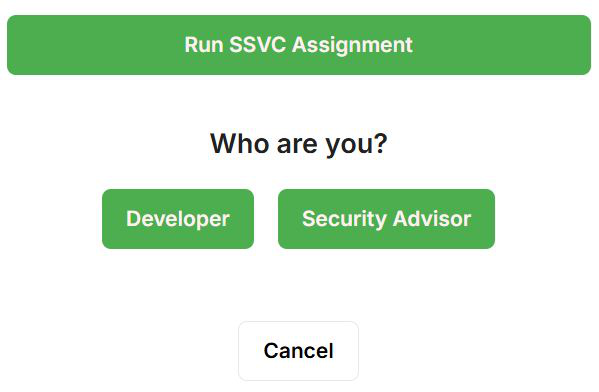
\includegraphics[scale=0.6]{resources/SSVC_Input.png}
    \caption{Interactive Decision Tree Interface: Initial role selection.}
    \label{fig:ssvc-tree-interface}
\end{figure}

Each response is processed to build a comprehensive recommended action plan, consisting of advisories such as \enquote{Apply patch immediately} when a vendor patch is available. Below is a code snippet demonstrating the logic for handling decisions within the tree structure and compiling the responses into a final recommendation. For example, one decision involves checking whether a vendor patch is available. Based on this, subsequent steps, such as applying the patch or exploring alternative mitigations, are determined.

\paragraph{Pseudocode for Decision Handling}
The following pseudocode demonstrates how decisions are processed to generate a recommendation:

\begin{verbatim}
// Generate recommendation based on patch availability
function generateRecommendation(data):
    recParts = []  // Collect recommendation parts

    if data.getPatchAvailableDev() == "yes":
        recParts.push("Vendor patch is available. Apply immediately.")
    else:
        recParts.push("No vendor patch found. Develop a custom fix.")

    return "Developer: " + recParts.join(" ")
\end{verbatim}

\paragraph{Final Recommendation}
After collecting all partial recommendations, the final message is composed and delivered (see example figure~\ref{fig:ssvc-recommendation}):

\begin{verbatim}
// Compile and deliver final recommendation
finalMessage = "Developer: " + recParts.join(" ")
setSuccessMessage(finalMessage)
onComplete(finalMessage)
\end{verbatim}

\begin{figure}[H]
    \centering
    
\includegraphics[width=0.8\linewidth]{resources/SSVC_Recommandation.png}
    \caption{Example of a final recommendation message delivered to a developer.}
    \label{fig:ssvc-recommendation}
\end{figure}

\subsection{Score Details Button}
A \textit{Show Score Details} popup (as described in section \ref{subsec:ui-explaining-score}) allows users to see the \ac{CVE}-ID, the \ac{CVSS} score and vector, the \ac{EPSS} score, the computed severity, and a textual explanation as described in section \ref{subsec:ui-explaining-score}. This is done through:

\begin{itemize}
  \item \textbf{Button Trigger:} A button in the \enquote{Vulnerability Details} view opens a modal dialog.
  \item \textbf{Dialog Contents:} The modal includes fields for the \ac{CVE} ID, \ac{CVSS} V3.1 base score, vector string, \ac{EPSS} metric, and the final severity. If any fields are missing, placeholders (e.g., \texttt{N/A}) or a note about further actions that can be taken are shown.
  \item \textbf{Hover Tooltips for Vectors:} Displays hover-based tooltips for each \ac{CVSS} vector attribute. When the user places the cursor over a specific field (e.g., \enquote{Attack Vector} or \enquote{Attack Complexity}), a concise explanation appears to clarify its impact on the vulnerability assessment.
  \item \textbf{Direct Link to the \ac{CVSS} Calculator:} Provides a direct link to the official \ac{CVSS} calculator.\footnote{\url{https://nvd.nist.gov/vuln-metrics/cvss/v3-calculator}} This link is automatically populated with the relevant vector data, allowing users to quickly review the existing metrics and explore different scoring scenarios.
\end{itemize}

This functionality is illustrated in figure~\ref{fig:score-details}, which shows an example of the \textit{Score Details} popup.

\begin{figure}[H]
    \centering
    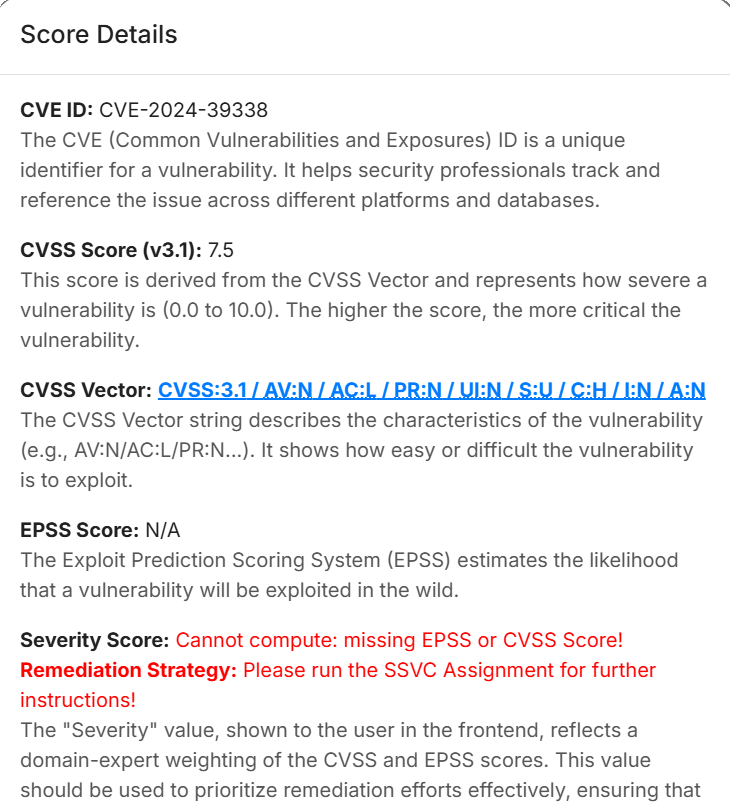
\includegraphics[scale=0.45, trim=2mm 2mm 2mm 2mm, clip]{resources/Score_Details_Button.PNG}
    \caption{Example of the \textit{Show Score Details} popup showing diverse data their explanation, and recommendations.}
    \label{fig:score-details}
\end{figure}

\section{Ranking and Prioritization Of All Vulnerabilities}
\label{sec:ranking-implementation}

This section describes the implementation of the model introduced in section~\ref{sec:rank-order-vulnerabilities}, focusing on how vulnerabilities are ranked and prioritized based on their severity.

\subsection{Descending Sort of Precalculated Severity Scores and Handling Missing Data}
The implementation takes the precalculated severity scores, which include contributions from \ac{CVSS} and \ac{EPSS}, and sorts them in descending order. This ensures that vulnerabilities with the highest severity scores are prioritized, while those with missing data are given placeholder scores for immediate attention.

For vulnerabilities with missing essential data, a placeholder score of \textbf{10.1} is assigned. This score exceeds the maximum valid severity of 10.0, ensuring these entries are sorted to the top of the list. In the user interface, such entries are highlighted with a pink \textbf{“UNKNOWN”} label, prompting users to investigate and resolve the missing information.

An example of the sorted list, as displayed in the user interface, is shown in figure~\ref{fig:rank-order-example}, where placeholder scores for missing data are indicated by a pink \enquote{UNKNOWN} label.

\begin{figure}[H]
    \centering
    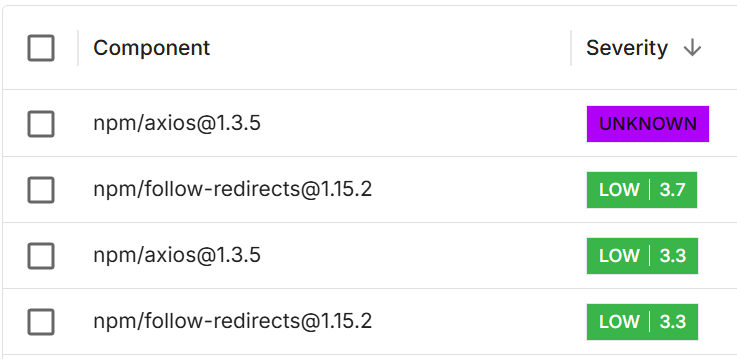
\includegraphics[scale=0.7]{resources/Rank-Order.PNG}
    \caption{Example of a sorted list of vulnerabilities in descending order of severity.}
    \label{fig:rank-order-example}
\end{figure}

\section{Conclusion}
\label{sec:implementation-conclusion}

The implementation details presented in this chapter show how the multi-dimensional vulnerability classification and remediation framework (see chapter~\ref{chapter:multidimensional-vulnerability-classification}) and the proposed system design (see chapter~\ref{chapter:design}) have been realized in a fully functional solution that integrates both backend and frontend components. Critical elements, such as caching and scheduled refresh (see section~\ref{subsec:caching-repository}), ensure that vulnerability data remains reliable, and continuously up-to-date, while minimizing external lookups.

The system interaction workflow (see section~\ref{subsec:system-interaction}) highlights how local \ac{OSV} data is leveraged, triggering external lookups for \ac{CVSS} and \ac{EPSS} only when strictly necessary. Building on these processes, the \ac{SSVC} endpoint (see section~\ref{par:ssvc-recommendation-endpoint}) and role-specific frontend logic (see section~\ref{sec:frontend-components}) enable targeted remediation recommendations for different user roles.

Moreover, combining \ac{CVSS} and \ac{EPSS} metrics captures both technical severity and exploitability factors in accordance with the multi-dimensional model. Finally, the ranking and visualization (see section~\ref{sec:ranking-implementation}) allow for effective prioritization of vulnerabilities, with any missing data explicitly flagged via a placeholder severity score (e.g., \textbf{10.1}). Taken together, these components form a cohesive, user-focused system that significantly streamlines vulnerability management and remediation activities, fulfilling the objectives outlined in earlier chapters.



\chapter{Evaluation}
\label{sec:evaluation}

This chapter evaluates the implemented system described in chapter~\ref{chapter:implementation} against the functional and non-functional requirements defined in chapter~\ref{chapter:requirements}, followed by an expert evaluation conducted through structured questionnaires to verify the system’s applicability and effectiveness.

\section{Evaluation of Functional Requirements}

This section reviews each functional requirement, detailing how the implemented solution meets each criterion with specific examples.

\begin{enumerate}
			
    \item \textbf{Multidimensional Vulnerability Classification Model (\ref{req:multidimensional_classification})}
    
    The implementation provides a multidimensional vulnerability classification by combining multiple vulnerability metrics into a unified severity score. For example, as described in section~\ref{subsec:severity-score}, \ac{CVSS} and \ac{EPSS} metrics are combined to produce an actionable severity rating. \textbf{This requirement is fulfilled.}
	      	      
    \item \textbf{Algorithm for Computing Vulnerability Classifications (\ref{req:classification_algorithm})}
    
    The implemented classification algorithm calculates severity scores using available metrics (section~\ref{subsec:severity-score}). This includes combining a weighted \ac{CVSS} score with a weighted \ac{EPSS} score to provide a clear and precise classification. \textbf{This requirement is fulfilled.}
	      	      
    \item \textbf{Remediation Recommendation Algorithm (\ref{req:remediation_algorithm})}
    
    The system generates tailored remediation recommendations using structured decision trees based on stakeholder roles, asset criticality, and patch availability (section~\ref{subsec:ssvc-integration}). For instance, a developer is provided recommendations like \enquote{Apply vendor patch immediately} if available or \enquote{Develop a custom mitigation} otherwise. \textbf{This requirement is fulfilled.}
	      
    \newpage
	                
    \item \textbf{Rank-Ordering Model for Vulnerabilities (\ref{req:vulnerability_ranking_model})}
    
    Vulnerabilities are ranked by their calculated severity, prioritizing the most critical vulnerabilities at the top (section~\ref{sec:ranking-implementation}). For example, vulnerabilities with higher computed severity scores appear prominently. \textbf{This requirement is fulfilled.}
	      	      
    \item \textbf{Interactive Score Explanation Interface (\ref{req:interactive_explanation})}
    
    The \enquote{Show Score Details} interface displays comprehensive vulnerability information, including \ac{CVE} identifiers, metrics, and an interactive, pre-filled link to the official \ac{CVSS} calculator. Interactive tooltips offer detailed explanations for terms like \enquote{Attack Vector} (section~\ref{sec:frontend-components}). \textbf{This requirement is fulfilled.}
	      	      
    \item \textbf{Handling of Missing Vulnerability Data (\ref{req:missing_data_handling})}
    
    When critical data is missing, the system assigns a placeholder severity score of 10.1, prioritizing the vulnerability at the top and visually highlighting it in pink with the label \enquote{UNKNOWN}. This prompts users to address incomplete data entries (section~\ref{sec:ranking-implementation}). \textbf{This requirement is fulfilled.}
	      	      
    \item \textbf{User Interface Warning for Missing Data (\ref{req:frontend_warning_missing_data})}
	      	      
    The user interface explicitly alerts users to missing data by highlighting vulnerabilities with a pink \enquote{UNKNOWN} label, communicating the need for immediate corrective actions (section~\ref{sec:ranking-implementation}). \textbf{This requirement is fulfilled.}
	      	      
    \item \textbf{Role-Based Decision Trees for Remediation (\ref{req:ssvc_decision_tree})}
	      	      
    Interactive decision trees guide stakeholders through remediation options tailored to context. For instance, developers answering questions about patch availability and asset criticality receive actionable steps like immediate patching or monitoring (section~\ref{subsec:ssvc-integration}). \textbf{This requirement is fulfilled.}
	      	      
    \item \textbf{Role-Specific Recommendations (\ref{req:role_specific_recommendations})}
	      	      
    The system provides explicit role-specific recommendations. Developers receive instructions such as \enquote{Apply patch immediately} (section~\ref{subsec:ssvc-integration}). \textbf{This requirement is fulfilled.}
	      	      
    \item \textbf{Caching Mechanism for External Data (\ref{req:data_caching_mechanism})}
	      	      
    Robust caching mechanisms significantly reduce external data retrieval. For instance, the system caches \ac{CVSS} vectors locally and performs efficient batch retrieval of \ac{EPSS} data (section~\ref{subsec:caching-repository}). \textbf{This requirement is fulfilled.}
	      
    \newpage
	      
    \item \textbf{Regular Data Synchronization (\ref{req:data_synchronization})}
	      	      
    A nightly synchronization cycle updates vulnerability data. Batch retrieval of \ac{EPSS} data and individual queries to external databases (\ac{NVD}) ensure data freshness, clearly illustrated by the scheduled refresh mechanism (section~\ref{subsec:scheduled-refresh}). \textbf{This requirement is fulfilled.}
	      	      
\end{enumerate}

\section{Evaluation of Non-Functional Requirements}

This section evaluates the non-functional requirements, emphasizing system quality, performance, and usability, and details how the implementation meets each requirement.

\begin{enumerate}
    
    \item \textbf{Modularity (\ref{nfr:modularity})}
	      	      
    The system distinctly separates backend functionalities (such as data caching, scheduled tasks, and repositories) from frontend interactions, facilitating maintainability. For instance, the repository layer manages data storage independently from the scoring algorithm and user interface logic (section~\ref{sec:backend-components}). \textbf{This requirement is fulfilled.}
	      	            
    \item \textbf{Scalability (\ref{nfr:scalability})}
	      	            
    Scalability is achieved through efficient batch-processing of external data (e.g., \ac{EPSS} batch requests) and a scheduled refresh mechanism to handle growing data volumes and simultaneous user interactions without performance degradation (section~\ref{subsec:scheduled-refresh}). \textbf{This requirement is fulfilled.}
	      	            
    \item \textbf{Usability (\ref{nfr:usability})}
	      	            
    The system provides a user-friendly interface featuring clear navigation, interactive decision trees, and comprehensive score explanations. Interactive components, such as tooltips and pre-filled links to external calculators, significantly enhance usability (section~\ref{sec:frontend-components}). \textbf{This requirement is fulfilled.}
	      	      
    \item \textbf{Compliance with External \ac{API} Rate Limits (\ref{nfr:rate_limit_compliance})}
	      	            
    The implementation responsibly manages external \ac{API} requests using caching and batching strategies, significantly reducing \ac{API} calls and thus reducing rate-limit violations. (section~\ref{subsec:caching-repository}). \textbf{This requirement is fulfilled.}
	      	      
    \item \textbf{Reliability and Error Handling (\ref{nfr:reliability_fallbacks})}
	      	            
    Robust error handling mechanisms are implemented. For instance, when critical data (\ac{CVSS} or \ac{EPSS}) is missing, the system assigns a placeholder severity score of \textbf{10.1}, prioritizing the vulnerability at the top and visually marking it as \enquote{UNKNOWN} to clearly communicate the issue (section~\ref{subsec:caching-repository}). \textbf{This requirement is fulfilled.}
	      	            
    \item \textbf{Maintainability (\ref{nfr:maintainability})}
	      	            
    The modular architecture and clear separation of backend layers (controller, service, data layers) enable straightforward maintenance and integration of future enhancements, such as additional data sources or scoring mechanisms (section~\ref{sec:backend-components} and section~\ref{sec:frontend-components}). \textbf{This requirement is fulfilled.}
    
\end{enumerate}

\section{Evaluation of Models by Domain Experts}

To further validate the practical relevance of the implemented framework, an expert evaluation was performed. Three domain experts from the field of cybersecurity assessed the applicability, clarity, and effectiveness of the models and algorithms presented in chapter~\ref{chapter:multidimensional-vulnerability-classification}. The evaluation was conducted using structured questionnaires provided in Appendix~\ref{appendix:questionnaire} and builds on the scientific foundations outlined in section~\ref{sec:scientific-foundations-questionnaire}.
\textit{Note: Expert statements have been partially paraphrased for clarity and brevity, while ensuring the original meaning was preserved.}

\subsection{Multi-Dimensional Classification Model}

Experts provided valuable feedback regarding the integration of \ac{CVSS} and \ac{EPSS} scores into a single unified severity score (see section \ref{sec:multi-dimensional-classification}). Expert feedback varied, with one expert explicitly stating: \enquote{I do not like merging \ac{CVSS} and \ac{EPSS}, as \ac{CVSS} is already considered in \ac{EPSS} according to page 2}. Another expert, however, emphasized the usefulness, stating: \enquote{The motivation to combine scores is clear and useful, although the selection of these two models specifically could be more clearly justified}.

Regarding weighting, suggestions included \enquote{a 50:50 ratio, initially not favoring one over the other,} while another expert preferred a heavier weighting towards EPSS (70\%) due to its empirical nature.

\textbf{Overall expert ratings (1 = very good, 6 = insufficient):}
\\
\begin{table}[H]
\centering
\begin{tabular}{|l|c|}
    \hline
    Expert & Rating \\
    \hline
    Expert 1 & 3 \\
    Expert 2 & 1 \\
    Expert 3 & 2 \\
    \hline
    \textbf{Average} & \textbf{2.0} \\
    \hline
\end{tabular}
\caption{Expert ratings for the Multi-Dimensional Classification Model}
\label{tab:expert_ratings_multidimensional}
\end{table}

\subsection{Algorithm to Compute Classification}

The algorithm's (see section \ref{sec:algorithm-classifications})  handling of missing data through placeholder scores was generally perceived positively, although concerns were raised. One expert noted: \enquote{The chosen placeholder could be confusing due to its proximity to valid score ranges; using infinity or NaN might be clearer}. Another expert commented positively: \enquote{As long as it is clearly indicated, it should not confuse users}.

Experts also identified instances where the computed severity might differ from organizational practices, such as vulnerabilities in unused library components without valid threat vectors.

\textbf{Overall expert ratings (1 = very good, 6 = insufficient):}
\\
\begin{table}[H]
\centering
\begin{tabular}{|l|c|}
    \hline
    Expert & Rating \\
    \hline
    Expert 1 & 2 \\
    Expert 2 & 1 \\
    Expert 3 & 1 \\
    \hline
    \textbf{Average} & \textbf{1.33} \\
    \hline
\end{tabular}
\caption{Expert ratings for the Algorithm to Compute Classification}
\label{tab:expert_ratings_algorithm_classification}
\end{table}

\subsection{Remediation Mechanism}

Experts confirmed that the \ac{SSVC}-inspired remediation model and algorithm (see sections \ref{sec:remediation_recommendation}, \ref{sec:algorithm-remediation}) generally aligns with real-world practices but highlighted some deviations. One expert stated: \enquote{Criticality of the asset is always considered, regardless of exploit likelihood}. Another emphasized: \enquote{Even if the criticality is low, vulnerabilities must be monitored and patched, as a single flaw can become critical in an attack chain}.

Decision factors identified as most critical by experts were \enquote{Exploit Likelihood and Asset Criticality, followed by Patch Availability}.

\textbf{Overall expert ratings (1 = very good, 6 = insufficient):}
\\
\begin{table}[H]
\centering
\begin{tabular}{|l|c|}
    \hline
    Expert & Rating \\
    \hline
    Expert 1 & 2 \\
    Expert 2 & 1 \\
    Expert 3 & 2 \\
    \hline
    \textbf{Average} & \textbf{1.67} \\
    \hline
\end{tabular}
\caption{Expert ratings for the Remediation Model (\ac{SSVC}-inspired)}
\label{tab:expert_ratings_remediation_ssvc}
\end{table}

\subsection{Rank-Ordering Mechanism}

All experts agreed prioritizing vulnerabilities based on the highest scores or incomplete data (see section \ref{sec:rank-order-vulnerabilities}) matches standard practice. One expert suggested improvements: \enquote{Grouping vulnerabilities by technology stack or business unit might offer better practical usability}. Another proposed: \enquote{A second queue for unknown-data vulnerabilities could avoid blocking immediate mitigation tasks}.

Experts also suggested further grouping based on the type of vulnerability: \enquote{Software flaws need to be sorted and categorized by cyber hygiene (e.g., misconfigurations), compliance (driven by regulations), quality (software 'convenience' patches), and security (software patches that fix vulnerabilities). All flaws need to be entered in a ticketing system and traced until solved}.

\textbf{Overall expert ratings (1 = very good, 6 = insufficient):}
\\
\begin{table}[H]
\centering
\begin{tabular}{|l|c|}
    \hline
    Expert & Rating \\
    \hline
    Expert 1 & 3 \\
    Expert 2 & 1 \\
    Expert 3 & 2 \\
    \hline
    \textbf{Average} & \textbf{2.0} \\
    \hline
\end{tabular}
\caption{Expert ratings for the Rank-Ordering Mechanism}
\label{tab:expert_ratings_rank_ordering}
\end{table}

\subsection{Overall Expert Feedback and Recommendations}
\label{subsec:overall_expert_feedback_recommendations}

Overall, the expert evaluation indicated that the integrated models effectively reflect common vulnerability management practices, providing useful mechanisms for classification, remediation, and prioritization. Experts highlighted the practicality and clear alignment with current industry approaches, with one expert noting explicitly: \enquote{These integrated models reflect well how we manage open-source vulnerabilities in practice.}

Nevertheless, the evaluation identified areas for further improvement, particularly regarding clearer communication of placeholder scores, and the inclusion of compliance as a key cybersecurity driver: \enquote{Compliance is one of the drivers for cybersecurity and must always be considered.} Additionally, experts suggested more granular grouping or filtering by technology stack or business units to enhance the usability of the rank-ordering mechanism. These considerations represent potential avenues for future enhancements of the framework.

\section{Summary}

This evaluation has demonstrated that the implemented system effectively meets all defined functional and non-functional requirements. The expert evaluation further validated the practical relevance and applicability of the multidimensional classification and remediation models, highlighting their alignment with common industry practices. Additionally, constructive feedback from domain experts identified opportunities for future enhancements, particularly concerning clearer communication of placeholder scores, improved grouping capabilities, and the integration of compliance considerations. Overall, the results confirm that the proposed solution provides a robust, scalable, and user-centric approach to vulnerability management.
\chapter{Conclusion and Outlook}
\label{chapter:conclusion-outlook}

This chapter summarizes the contributions and findings of the thesis, highlighting its significance and limitations. Additionally, it outlines potential avenues for future research that could further enhance the proposed multidimensional vulnerability management framework.

\section{Conclusion}
This thesis proposed a multidimensional framework for the classification and remediation of vulnerabilities, aimed at addressing identified shortcomings within the existing vulnerability management component of \ac{SCA} Tool developed by the \ac{OSS} group at \ac{FAU}. The existing approach, which relies exclusively on the \ac{CVSS}, exhibits notable limitations, particularly inconsistencies among security practitioners' scoring and a lack of empirical exploitation data \autocite{spring_time_2021}. To overcome these limitations, the proposed framework integrates technical severity metrics from \ac{CVSS} with empirical exploit probability data provided by \ac{EPSS}, thus offering a more holistic and context-aware method for vulnerability prioritization.

An evaluation against functional and non-functional requirements demonstrated that the proposed framework conceptually addresses all stated criteria, showing strong potential in enhancing vulnerability prioritization and remediation processes. Moreover, an expert evaluation confirmed the framework's practical relevance and its alignment with current industry standards and best practices. Experts highlighted particularly the advantage of integrating empirical exploitability measures alongside structured, stakeholder-specific remediation decision processes based on the \ac{SSVC} framework.

However, the evaluation also revealed areas for further refinement. The method of combining \ac{CVSS} and \ac{EPSS} metrics elicited differing perspectives, with some experts noting conceptual overlaps that could potentially complicate interpretation. Additionally, the explicit integration of compliance aspects was recommended as a crucial extension to ensure alignment with organizational cybersecurity strategies.

In summary, the thesis conceptually advanced vulnerability management methodologies by proposing a comprehensive multidimensional classification and remediation framework. Its validation by domain experts underscores its potential effectiveness and practical applicability, while also highlighting avenues for further improvement.

\section{Outlook}
Several avenues for future research emerge from the presented framework and its evaluation:

\paragraph{Evaluation Against Ground Truth Data} An important next step would be the empirical validation of the proposed classification framework against ground truth data. Evaluating the proposed model against datasets containing historically verified cases of exploited vulnerabilities would provide a robust empirical foundation for assessing the predictive accuracy and reliability of the integrated \ac{CVSS} and \ac{EPSS} classification approach.

\paragraph{Explicit Incorporation of Compliance Considerations}
Integrating \\ compliance-driven factors, such as adherence to standards like \ac{GDPR} or ISO 27001, into the vulnerability assessment and prioritization model would ensure a more holistic and strategically aligned approach. \ac{GDPR} imposes strict regulatory obligations on organizations within the \ac{EU} to protect personal data \autocite{chassang_impact_2017}. Therefore, future research could explore explicitly identifying and prioritizing vulnerabilities affecting systems that process sensitive personal data, aligning vulnerability management more closely with these regulatory requirements. Similarly, the ISO 27001 standard provides a systematic framework for assessing and managing information security risks, including regular evaluation and prioritization of business-critical assets \autocite{international_organization_for_standardization_iso_isoiec_2018}. Integrating ISO 27001 risk assessments into the proposed vulnerability classification framework would ensure that vulnerabilities affecting high-risk assets, as defined by organizational security policies, receive higher prioritization. Consequently, this explicit incorporation of compliance considerations would enhance the alignment between technical vulnerability management and broader organizational information security and regulatory strategies.

\paragraph{Advanced Grouping and Filtering Capabilities}
Lastly, introducing more granular grouping and filtering functionalities - such as by business units, technology stacks, or organizational responsibilities - could significantly enhance the practical usability of the framework. This would allow organizations to tailor vulnerability management more precisely to their specific operational contexts and strategic priorities.

These suggested research directions would contribute to refining the conceptual framework, ultimately fostering more effective and strategically aligned approaches to vulnerability classification and remediation.


%%%%%%%%%%%%%%%%%%%%%%%%%%%%%%%%%%%%%%%%%%%%%%%%%%%%%%%%%%%%%%%%%%%%%%%%%%%%


%%%%%%%%%%%%%%%%% CLOSING SECTIONS %%%%%%%%%%%%%%%%%%%%%%%%%%%%%%%%%%%%%%%%%

\begin{appendices}

  \renewcommand{\setthesection}{\Alph{section}}
  \renewcommand{\thesection}{\Alph{section}}
  \headerstyleclosingsection\
  \renewcommand\sectionmark[1]{\markright{\thesection : #1}} % Appendix A. => Appendix A:

  \input contents/appendices.tex
\end{appendices}

\cleardoublepage
\renewcommand\bibname{\referencesname}
\addcontentsline{toc}{chapter}{\referencesname}
\printbibliography
%%%%%%%%%%%%%%%%%%%%%%%%%%%%%%%%%%%%%%%%%%%%%%%%%%%%%%%%%%%%%%%

\end{document}
